\documentclass{tudelft-report}

\usepackage{pdfpages}
\usepackage[export]{adjustbox}
\newcommand{\reqr}[1]{{\noindent\emph{#1:}}}
\usepackage{algorithm}
\usepackage{algpseudocode}
\usepackage{float}

\begin{document}

%% Use Roman numerals for the page numbers of the title pages and table of
%% contents.
\frontmatter

\title[TI3800 Bachelorproject]{Peer Matching Tool}
\author{Floris Verburg \and Freek van Tienen \and Marijn Goedegebure}
\affiliation{Technische Universiteit Delft}
\coverimage{coverimage.png}
\makecover

%% Include an optional title page.
\begin{titlepage}

\begin{center}

%% Insert the TU Delft logo at the bottom of the page.
\begin{tikzpicture}[remember picture,overlay]
    \node at (current page.south)[anchor=south,inner sep=0pt]{
        
\includegraphics{cover/logo}
    };
\end{tikzpicture}

%% Extra whitespace at the top.
\vspace*{2\bigskipamount}

%% Print the title in cyan.
{\makeatletter
\titlestyle\color{tudelft-cyan}\Huge\@title
\makeatother}

%% Print the optional subtitle in black.
{\makeatletter
\ifx\@subtitle\undefined\else
    \bigskip
    \titlefont\titleshape\LARGE\@subtitle
\fi
\makeatother}

\bigskip
\bigskip

by
%door

\bigskip
\bigskip

%% Print the name of the author.
{\makeatletter
\titlefont\Large\bfseries\@author
\makeatother}

\vfill

in partial fulfilment of the requirements for the degree of
%in overeenstemming met de vereisten voor het verkrijgen van de graad van

\bigskip
\bigskip

{\bfseries Bachelor of Science}

in Computer Science

\bigskip
\bigskip

at the Delft University of Technology,
%aan de Technische Universiteit Delft,

to be defended on Tuesday June 24, 2014 at 10:00 AM.
%in het openbaar de verdedigen op dinsdag 1 januari om 10:00 uur.

\vfill

\begin{tabular}{lll}
%% Add additional information here, per faculty requirements, e.g
%    Student number: & 1234567 \\
%    Project duration: & \multicolumn{2}{l}{March 1, 2012 -- January 1, 2013} \\
    Supervisor: & Prof. drs. dr. L.J.M. Rothkrantz\\
    Thesis committee:
        & Prof. drs. dr. L.J.M. Rothkrantz \\
        & Dr. ir. D. Datcu\\
        & M.A. Larson
\end{tabular}

%% Only include the following lines if confidentiality is applicable.
\bigskip
\bigskip
%\emph{This thesis is confidential and cannot be made public until December 31, 2013.}
%\emph{Op dit verslag is geheimhouding van toepassing tot en met 31 december 2013.}

\bigskip
\bigskip
An electronic version of this thesis is available at \url{http://repository.tudelft.nl/}.
%Een elektronische versie van dit verslag is beschikbaar op \url{http://repository.tudelft.nl/}.

\end{center}

\end{titlepage}



\chapter*{Summary}
\setheader{Summary}

Massive open online courses (MOOCs) all around the world are growing in size. 
Therefore, the practical assignments need to be easy to manage.
The growth also means that it is more difficult for each participant to find a possible practical partner due to the large amount of people.
The difficulty to find the correct partner or group members when the students do not see each other during courses and have not even met most of the people from the course is also affected.

For this Bachelor Project we have improved upon this process by creating an application that can be used to create practical groups without the participants being required to go search intensively trough all the participants.
Participants are able to easily access the application, fill in some relevant information about themselves and then get recommendations of possible practical partners or group members.

We have divided the project in three phases:
\begin{itemize}
\item Research and set-up (phase 1)
\item Design and implementation (phase 2)
\item Testing, documentation and presentation (phase 3)
\end{itemize}
Each of these phases describes the things that need to be done during that phase.

During the implementation phase we used a known software development framework.
This development framework is known as scrum.
Scrum is based on the agile software development framework which can be used to 
manage software projects.

We use the Play framework for the developing of the application. 
The Play framework gives us the possibility to easily create a web application using Java.
This frameworks follows the Model View Controller (MVC) architectural pattern applied to the Web architecture.

For our matching algorithm we used our custom designed algorithm.
This algorithm uses the skills defined by the user and the teacher to find the best matching with the preferences of the teacher.


Creating code with good quality, maintainability and extendability of the system was important during the project.
We achieved this using several tools, like Findbugs and Checkstyle.

Another important aspect of the project was testing the code.
We have performed different kind of tests to ensure good functioning code.

During the implementation phase, we already started with testing. Because the system was not completed during this phase, only parts of the system could be tested.
We performed different kind of unit tests to provide a basic code coverage.
We also used continuous integration, which executed the tests ever time we pushed our code to git.
Besides the unit tests we have performed integration tests to ensure the connection between the different components.

The testing of the entire system is done after the implementation phase has been completed. This is partly done by checking if the final product matches the requirements set. It is also done by letting the target audience use the system and document the findings.

A working beta implementation of the complete system has been delivered as a proof of concept and most of the initially set requirements were fulfilled.


\chapter*{Preface}
\setheader{Preface}

This report is the final report which concludes the development of a Peer Matching Application for Practicals for Massive Open Online Courses (MOOCs).
This project was executed for the TI3800 - Bachelor Project course at the Delft University of Technology in the Netherlands.
The assignment was issued by Prof. Drs. Dr. L.J.M. Rothkrantz, also from the Delft University of Technology.
\\\\
The project began at April 21st 2014 and finished at June 24th 2014. All research and development took place at the Delft University of Technology, department of Electrical Engineering, Mathematics and Computer Science. This report will provide examines the assignment, requirements, project methodology, system design, implementation, testing and results of the project.
\\\\
We would like to thank the following persons in particular:
\begin{itemize}
\item Leon Rothkrantz, for supervising the project and providing support and valuable guidance throughout the process.
\item Dragos Datcu, for supervising the project and providing support and valuable guidance throughout the process.
\item Felienne Hermans, for coordinating the Bachelor Project course and attending our final presentation.
\item Martha Larson, for coordinating the Bachelor Project course.
\end{itemize}

\begin{flushright}
{\makeatletter\itshape
    \@author \\
    Delft, June 2014
\makeatother}
\end{flushright}



\tableofcontents

%% Use Arabic numerals for the page numbers of the chapters.
\mainmatter

\chapter{Introduction}

\section{Problem Description}
It is well known that many students come to the University to visit lectures because it provides the opportunity to meet peers and to have discussions also about less academic topics. 
The meeting place at the University is partly replaced by a virtual meeting place. 
Students report about their daily activities, opinions, problems using social media. 
\\\\
At this moment social media play a limited role in the academic process of teaching and learning. 
But social media offer great opportunities, especially around the development of MOOCS (Massive Open Online Courses). 
\\\\
The basic idea of MOOCS is that students remote in place and time follow the lectures, they can use social media as academic communication media, where students discuss about their study activities, put forward their questions and get help and support from peers. 
\\\\
The question is how to find the best matching peers especially peers outside TUDelft. 
Inspecting all the profiles via Facebook is too time consuming. 
Supporting matching tools are needed. 
\\\\
At this moment there many sites finding the best matching partner, our interest is finding the best matching study partners. 
A possible option is to extract features from student profiles via Facebook, take care of preferences and expert knowledge and train classifiers or other matching technologies.

\section{Target}
In this project, we focus mainly on students, but teachers are also important for accomplishing a good result.
We need to match the students based on their skills, but the teachers are the ones that determine the demands for the assignments and what the optimal level of average skills in a group is.
\\\\
We focus on creating optimal practical groups for students.
So it is also very important to test the application with these people.

\section{Outline}
We will identify the assignment based on the requirements we determined in chapter 2. 
In this chapter, we also give an impression on how the application will look like by means of graphical user interface (GUI) mockups.
\\\\
Then, in chapter 3 the strategy and methodology of the process will be explained by going into more detail on our approach, the project planning and tools used throughout the project.
\\\\
Next, in chapter 4 the implementation details and design decisions will be explained.
We will discuss why we chose for certain implementations of for example the algorithm or the system design.
\\\\
In chapter 5 we will discuss our way of testing. 
We differentiate the unit testing and the user testing.
\\\\
Finally, we conclude the report in chapter 6 by evaluating the results and providing suggestions for future work.
\\\\
After the conclusion a Bibliography and several Appendices can be found. 
These appendices contain intermediate products and more detailed descriptions that are referred to in the text in order to improve the readability of the main report.


\chapter{Assignment and Requirements}

\section{Assignment Summary}
The whole original assignment can be found in Appendix B. In this section we just provide a short summary of the assignment. 

Massive open online courses (MOOCs) around the world are growing in size and thus the practical assignments need to be easy to manage.
The growth also means that it is more difficult for each participant to find a possible practical partner due to the large amount of people.
It also becomes really difficult to find the correct partner or group members when you don't see each other during courses and haven't even met most of the people from your course.

Most of the time participants of MOOCs are searching group members on social media like Facebook or Twitter.
They just try to look through some of the participants names in the course, search for them on-line through social media and check if they are a capable partner or group member.
This approach takes a lot of time and most of the time there are too much MOOC participants to go trough all of them.

Next to the fact that this process is very time consuming, this process also often leads to a sub optimal solution.
This is due to the problem that people often look for partners of group members which share the same interests.
While this often makes it easy to work together, this will not guarantee that you have a good functioning group and enough knowledge inside the group.

We would like to improve upon this process by creating an application that can be used to create practical groups without the participants being required to go search intensively trough all the participants.
Participants should be able to easily access the application, fill in some relevant information about themselves and then be recommended possible practical partners or group members.

The interaction with the system has some difficulties.
If we want to get some information from third parties, we are required to use the information in a way this third party delivers the data.
There can be difficulties processing this data.

The recommendation of possible group members can be quite difficult too.
One of the problems we are facing is the question: What user information is useful to determine whether two people can be good practical partners?

\section{Client and academic supervision}
During the project, we had both a TU Delft coach and a company contact.
During weekly meetings, we discussed our progress and the preferences form the client.
In Table~\ref{supervision} you can see the roles of our supervisors.

\begin{table}[H]
\begin{tabular}{ | p{3cm} | p{5cm} | p{6cm} | }
 \hline
Leon Rothkrantz & Group Mentor and Supervisor & Supervises the project from the academic point of view and aides the group with difficulties.\\ \hline
Dragos Datcu &  Client, Group Mentor and Supervisor & Supervises the project from a client point of view and aides the group with difficulties.\\
\hline
\end{tabular}
\caption{Our supervisors}
\label{supervision}
\end{table}

\section{Actors of the System}
The system can be used by three different actors.
Each of these actors can perform different actions and therefore have different requirements.
By defining the requirements, as we do in the next section, we take these different actors in account.

\subsubsection{Actor 1: MOOC participant}
Due to the nature of the MOOCs, there are no requirements set for the participants.
Every person with an interest in the given course can enlist for the MOOC and should thus be able to register with our system.
\subsubsection{Actor 2: MOOC teacher/MOOC administrator} 
The MOOC is organised by a professor of an university.
This professor will need to register with the system and create a MOOC.
\subsubsection{Actor 3: Groups of participants}
This actor consist of two or more MOOC participants who accepted each other to their group.
These groups can be of variable size, set by the MOOC organiser.

\section{Global Goals and Requirements}
To determine the direction the project should be following, we define goals for the project.
These goals will later be used to determine whether the final product is in line with these goals.
\begin{itemize}
\item The final product, that will be presented, will be a working proof of concept which will fit closely with the specified target audience and demands of the assignment.
\item We want to create a platform for searching other students, letting the students invite other students for a practical group and letting the students join each other.
\item We want the final product to recommend good fitting, possible group members to the students.
By "good fitting" we mean that there is some heuristic that we use to calculate whether two students would make a good combination.
\item We want the final product to achieve more optimal groups than the current situation by recommending other students.
\end{itemize}

The goals do not include a goal for the teachers part, because the current goals focus on the student.
This is because of the limited time of the project and the current goals having enough depth for an extensive system.
Next to this, the assignment specifically focusses on the need of the students to have a platform to search, interact with other students to form practical groups and have help with searching for their best practical group.
Although it would be beneficial for the teacher to have an easy to use platform for managing his practical assignments, it is out of the scope of this project.

To provide an overview of what actions the software must be capable of, we define four global requirements for the system.
By defining these three global requirements we provide a foundation for the detailed requirements.
\begin{itemize}
\item MOOC teachers must be able to create, manage and edit courses.
Participants of their MOOC are able to register to this course.

\item MOOC students must be able to register and deregister for a course.

\item The system must be capable to use personal data provided by the user to find a suggestion of an appropriate practical partner or group member.
It must be possible to adjust the definition (parameters) of the appropriate practical partner or group member, and search trough several suggestions.
\end{itemize}

\section{Detailed Requirements}
This section will mention the different requirements that involve the basic system which the actors interact with.
The section starts with mentioning the possible types of user information the application can use and what requirements are associated with that.
Followed up by what actions are possible within the system.
After that, the kind of system is limited by the requirements listed.
Lastly we will list the requirements set for the algorithm.

We use the MoSCoW model to divide the requirements in their appropriate categories.
The M stands for must have, the S for should have, the C for could have and the W for would have.

\subsection{User Information}
\begin{tabular}{ | p{0.5cm} | p{12cm} | p{2cm} | }
\hline
\textbf{\#} & \textbf{Requirement} & \textbf{MoSCoW} \\ \hline
1 & Users must have a viewable profile that can be filled with personal information. & M \\ \hline
2 & Users must be able to enter the following registration information during registration: Full name, Email address, Password. & M \\
3 & Users must fill in their academic performances. Which knowledge, skills and completed courses does the user have? & M \\ \hline
4 & Users should be able to enter the basic user information, like: country, age, short description, skills, education, a picture and personality traits. & S \\ \hline
5 & Users could be able to use a personality test to determine their personality traits. & C \\ \hline
6 & Users could be able to fill in their personality traits. & C \\ \hline
7 & Users could be able to enter the following extended user information: preferred group role, role of the other group members, etcetera. & C \\ \hline
8 & Users could be able to enter a predefined questionnaires. & C \\
\hline
\end{tabular}

\subsection{Usage of the System}
\begin{tabular}{ | p{0.5cm} | p{12cm} | p{2cm} | }
\hline
\textbf{\#} & \textbf{Requirement} & \textbf{MoSCoW} \\ \hline
\multicolumn{3}{|p{14.5cm}|}{\textbf{Actor 1: MOOC participant}} \\ \hline
1 & The potential participant (anyone who visits the site) must be able to view the different MOOCs without registering or logging in. & M \\ \hline
2 & The participant must be able to inform him/herself about the usage of the application without registering or logging in. & M \\ \hline
3 & The participant must be able to register to the application. & M \\ \hline
4 & The participant must be able to log in to the application. & M \\ \hline
5 & The participant must be able to register to the MOOCs which they were enlisted for (known to the administrator). & M \\ \hline
6 & The participant must be able to view a possible practical partner. & M \\ \hline
7 & The participant must be able to communicate with the possible practical partner to verify the matching. & M \\ \hline
8 & The participant must be able to accept or decline the practical partner into his practical group. & M \\ \hline
9 & The participant must be able to communicate within the group. & M \\ \hline
10 & The participant should be able to ask a currently existing group if he can join them. & S \\ \hline
11 & The participant should be able to use their LinkedIn profile to log in to the application. & S \\ \hline
12 & In case the participant already has an account, the participant should be able to add the course to his profile using the teachers url. & S \\ \hline
13 & The participant should be able to receive an invitation from a group. & S \\ \hline
14 & The participant should be able to accept the invitation from a group. & S \\ \hline
15 & The participant could be able to set his preferences for his possible partner. & C \\ \hline
16 & The participant could be able to search for other participants using information that is available in the profile. & C \\ \hline
\end{tabular}
\begin{tabular}{ | p{0.5cm} | p{12cm} | p{2cm} | }
\hline
\multicolumn{3}{|p{14.5cm}|}{\textbf{Actor 2: MOOC teacher/MOOC administrator}} \\ \hline
17 & The administrator must be able to create a course and add this to his account. & M \\ \hline
18 & The administrator must be able to create an url that he can use to invite the participants. & M \\ \hline
19 & The administrator must be able to manage the list of participants and groups of participants. & S \\ \hline
20 & The administrator must be able to open and close the participant registration for a course. & S \\ \hline
21 & The administrator should be able to set a deadline for a practical. & S \\ \hline
22 & The administrator should be able to communicate with every participant. & S \\ \hline
23 & The administrator should be able to communicate with the groups. & S \\ \hline
24 & The administrator should be able to grade the group for its practical. & C \\ \hline
25 & The administrator could be able to provide for his own criteria for each of his course. & C \\ \hline
26 & The administrator could be able to add different assignments to the application. & C \\ \hline
27 & The administrator could be able to view what groups have finished what assignments. & C \\ \hline
28 & The administrator could be able to grade the different assignments. & C \\ \hline
29 & The administrator could be able to provide feedback for the different assignments. & C \\ \hline
\end{tabular}
\begin{tabular}{ | p{0.5cm} | p{12cm} | p{2cm} | }
\hline
\multicolumn{3}{|p{14.5cm}|}{\textbf{Actor 3: Groups of participants}} \\ \hline
30 & A group should be able to view a possible group member. & S \\ \hline
31 & A group should be able to invite a possible group member to join their group. & S \\ \hline
32 & A group should be able to accept an request from a participant to join their group. & S \\ \hline
33 & The groups must be able to communicate with each other using the application. & C \\ \hline
34 & The group could be able to select their preferences for the new group member. & C \\ \hline
35 & The participants could be able to share files to other group members using this application. & C \\ \hline
36 & The participants would be able upload their source code to the application for verification. & W \\
\hline
\end{tabular}

\subsection{Kind of System}
\begin{tabular}{ | p{0.5cm} | p{12cm} | p{2cm} | }
\hline
\textbf{\#} & \textbf{Requirement} & \textbf{MoSCoW} \\ \hline
1 & The application must be easily accessible to both participants and course organizers. & M \\ \hline
2 & The system must provide account management functionality. & M \\ \hline
3 & The system must use a database to store the different data put in by the user. & M \\ \hline
4 & The system could be able to be combined with practical systems already used by MOOC organizers. & C \\
\hline
\end{tabular}

\subsection{Peer Matching}
\begin{tabular}{ | p{0.5cm} | p{12cm} | p{2cm} | }
\hline
\textbf{\#} & \textbf{Requirement} & \textbf{MoSCoW} \\ \hline
1 & The algorithm must be able to use a list of users as input. & M \\ \hline
2 & The algorithm must deal with continuous variation in amount of users. & M \\ \hline
3 & The algorithm must be able to return one or more suggestions of practical partners to the user given a list of rejected users. & M \\ \hline
4 & The algorithm must be able to return one or more suggestions of possible groups the participant could join. & M \\ \hline
5 & The algorithm uses basic user provided data (e.g. education, preferences) to build up a profile for a course participant. & S \\ \hline
6 & The algorithm can calculate whether two people will be good practical partners using the basic user provided data. & S \\ \hline
7 & The algorithm can return a possible practical partners using the basic user provided data. & S \\ \hline
8 & The algorithm uses advanced user provided data (e.g. asked questions, programming tests) to build up an extended profile for a course participant. & C \\ \hline
9 & The algorithm can calculate whether two people will be good practical partners using the advanced user provided data. & C \\ \hline
10 & The algorithm can return a possible practical partner using the basic user provided data. & C \\ \hline
11 & The algorithm could be able to respond to the preferences of groups. & C \\ \hline
12 & The algorithm could be able to respond to the preferences of a participant. & C \\ \hline
13 & The algorithm would have to be able to use information gathered from rejections to improve the matching. & W \\
\hline
\end{tabular}

\section{Changed requirements}
During the project we noticed that some requirements were not classified properly.
These requirements do not have the priority that we initially thought they would have.
Following the goals that we have set for the final product, we reasoned that these requirements were not must haves for the final product.
The teacher part of the system is something we would want to look into, the moment that the final product has a focus towards actual use and not at the proof of concept phase.
Below we listed the requirements that were reclassified.
We have listed both the old and new classification.
\begin{tabular}{ | p{0.5cm} | p{10cm} | p{2cm} | p{2cm} | }
\hline
\textbf{\#} & \textbf{Requirement} & \textbf{Old MoSCoW classification} & \textbf{New MoSCoW classification} \\ \hline
19 & The administrator must be able to manage the list of participants and groups of participants. & M & S \\ \hline
20 & The administrator must be able to open and close the participant registration for a course. & M & S \\ \hline
33 & The groups must be able to communicate with each other using the application. & M & C \\ \hline
\end{tabular}



\section{Graphical User Interface Mockups}
We have multiple important features in our application.
Each of these features has an own graphical user interface (GUI).
Below, we will provide mockups from the graphical user interfaces of the most important features.

\subsection{Profile}
As you can see in Figure~\ref{mockup_profile}, you can view someone's (or your own) profile.
You can see the basic profile information which the user has filled in himself.

If you are looking for a practical partner, you can get a better impression of that person when you get an overview of the profile information of that person.
This is just a simple page, because you should quickly get an impression of the student.\\

\begin{figure}[H]
    \centering
    \captionsetup{justification=centering}
    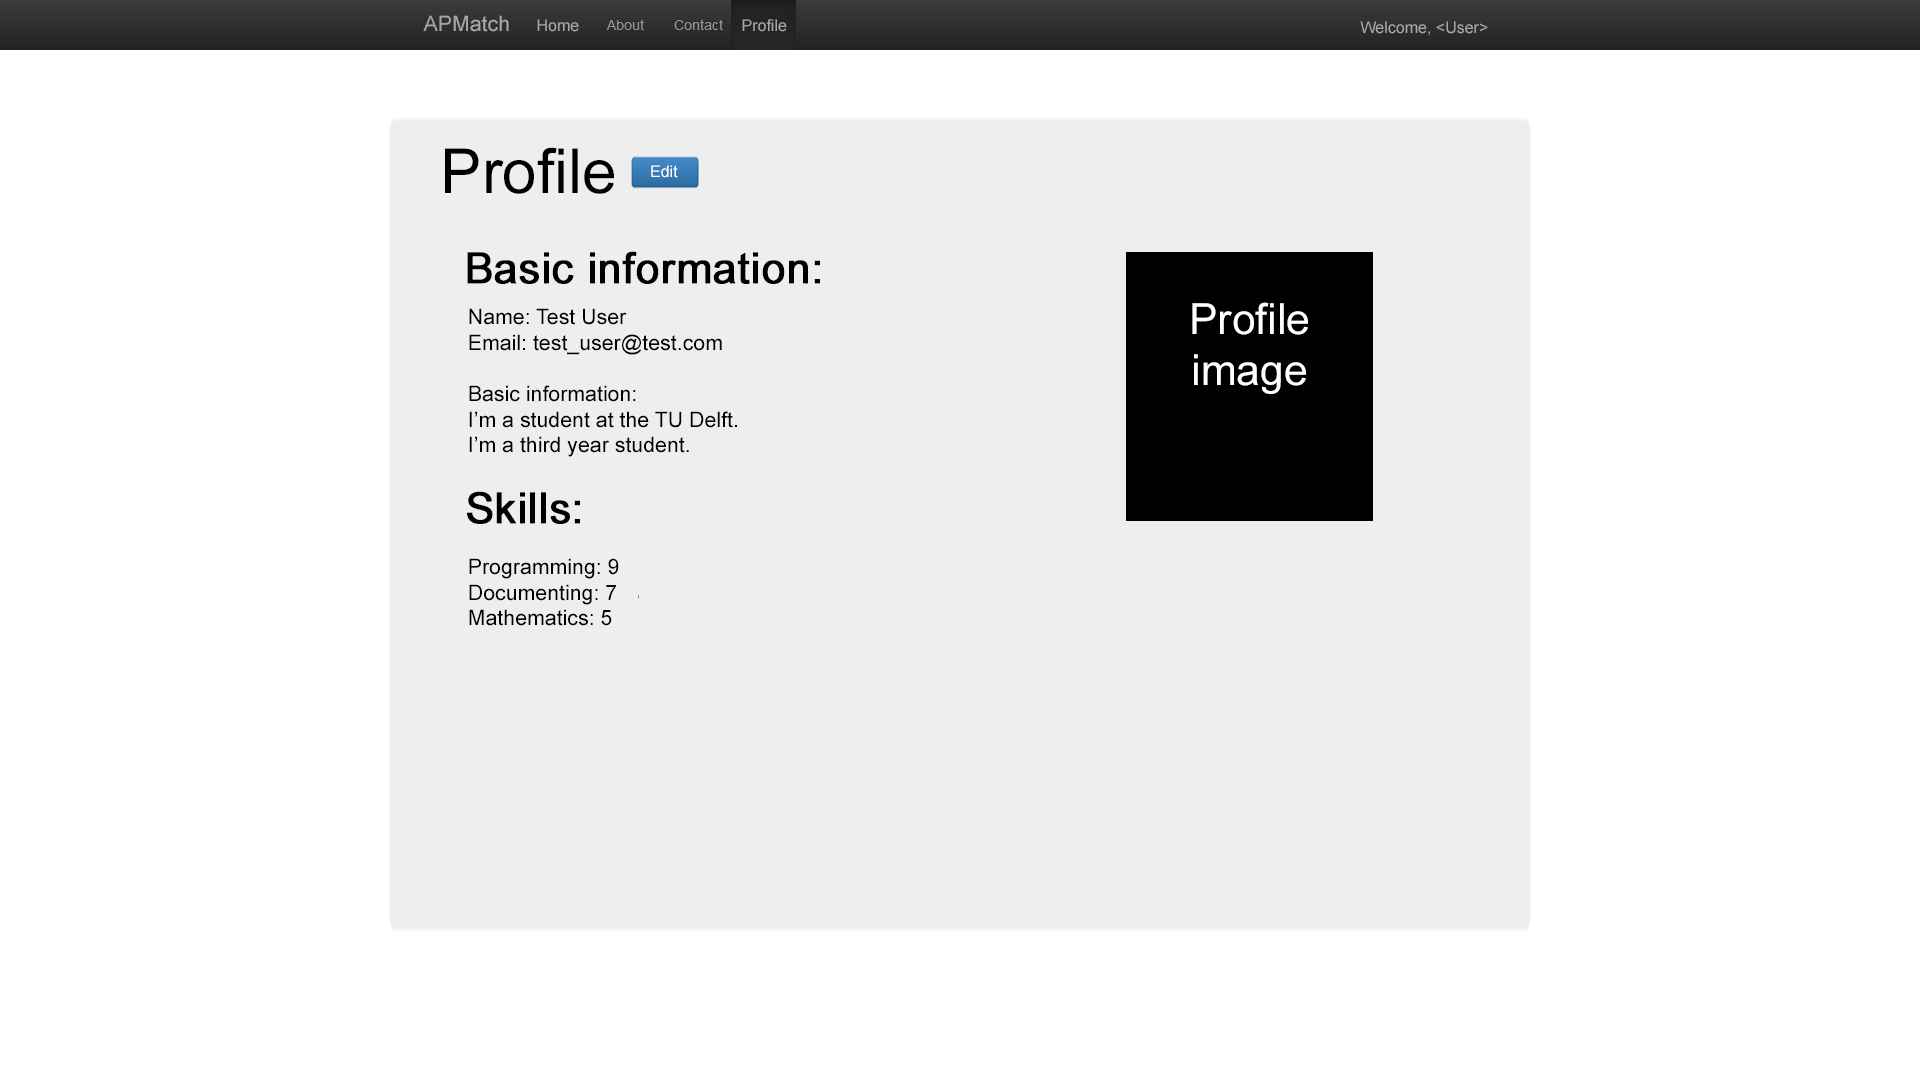
\includegraphics[width=\textwidth, frame]{images/mockup_profile}
    \caption{Interface for the profile page}
    \label{mockup_profile}
\end{figure}

In Figure~\ref{mockup_edit_profile}, you see the page for editing your profile.
On this page, you can edit your basic profile information as well as the level of your skills.
You can also change your password and your profile image.
This information will be taken into account while determining the recommended practical partners.
So it is important for the users to be able to fill in this information easily.

\begin{figure}[H]
    \centering
    \captionsetup{justification=centering}
    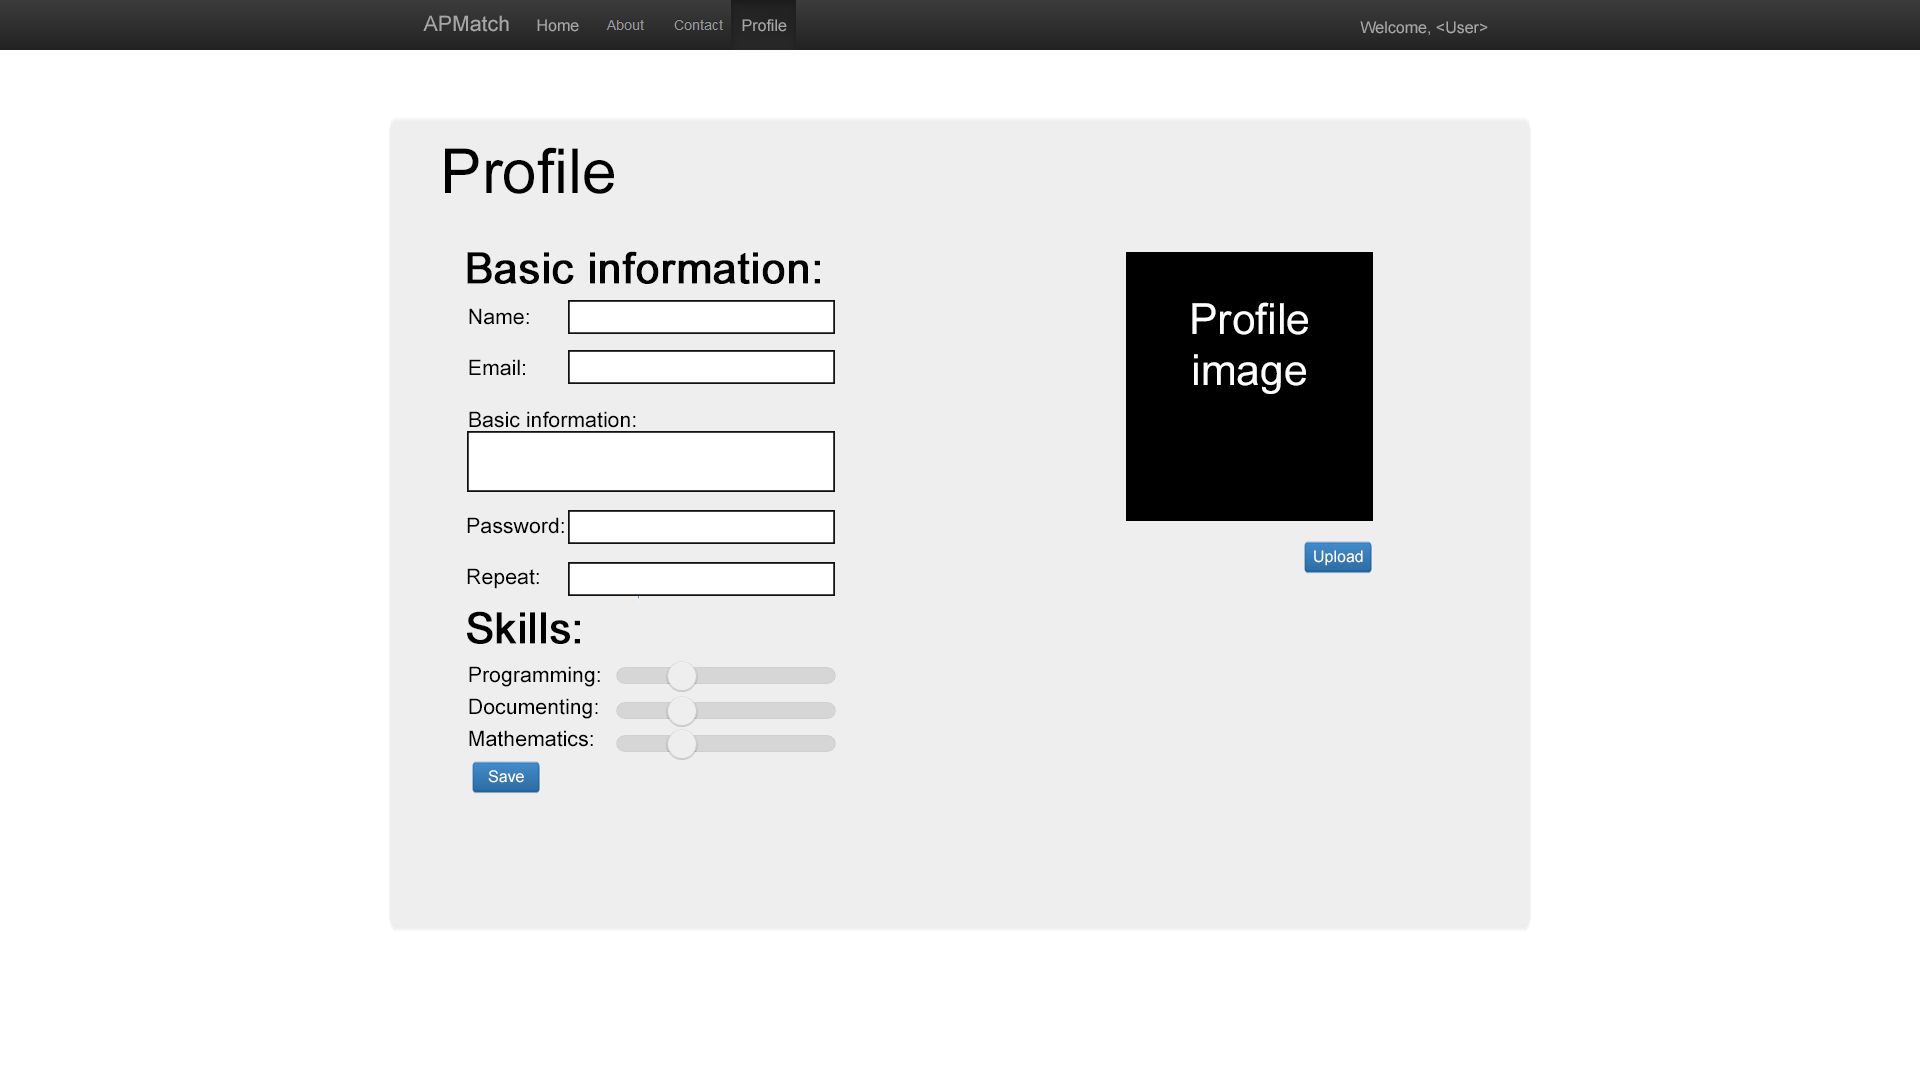
\includegraphics[width=\textwidth, frame]{images/mockup_edit_profile}
    \caption{Interface for editing the profile}
    \label{mockup_edit_profile}
\end{figure}

\subsection{Practical}
The main feature in our application is recommend practical partners.
Therefore, the users need to be able to register for a practical assignment.
The users receive a link from the teacher and when they have clicked on it, the user is added to the practical.
The practical is then added to the user's practical overview.
Such an overview can be seen in Figure~\ref{mockup_practical_overview}

In Figure~\ref{mockup_practical}, the user can see a page for a certain practical.
First of all, there is some information about the practical itself.
We show a short description of the practical.

After that, we show the most important part, the recommendation.
The application determines which other practical groups matches your group the best.
On this page you can click on the practical group for more information.
You can also invite a practical group to join yours.

After the recommendation part, we also show the user's current practical group.


\begin{figure}[H]
    \centering
    \captionsetup{justification=centering}
    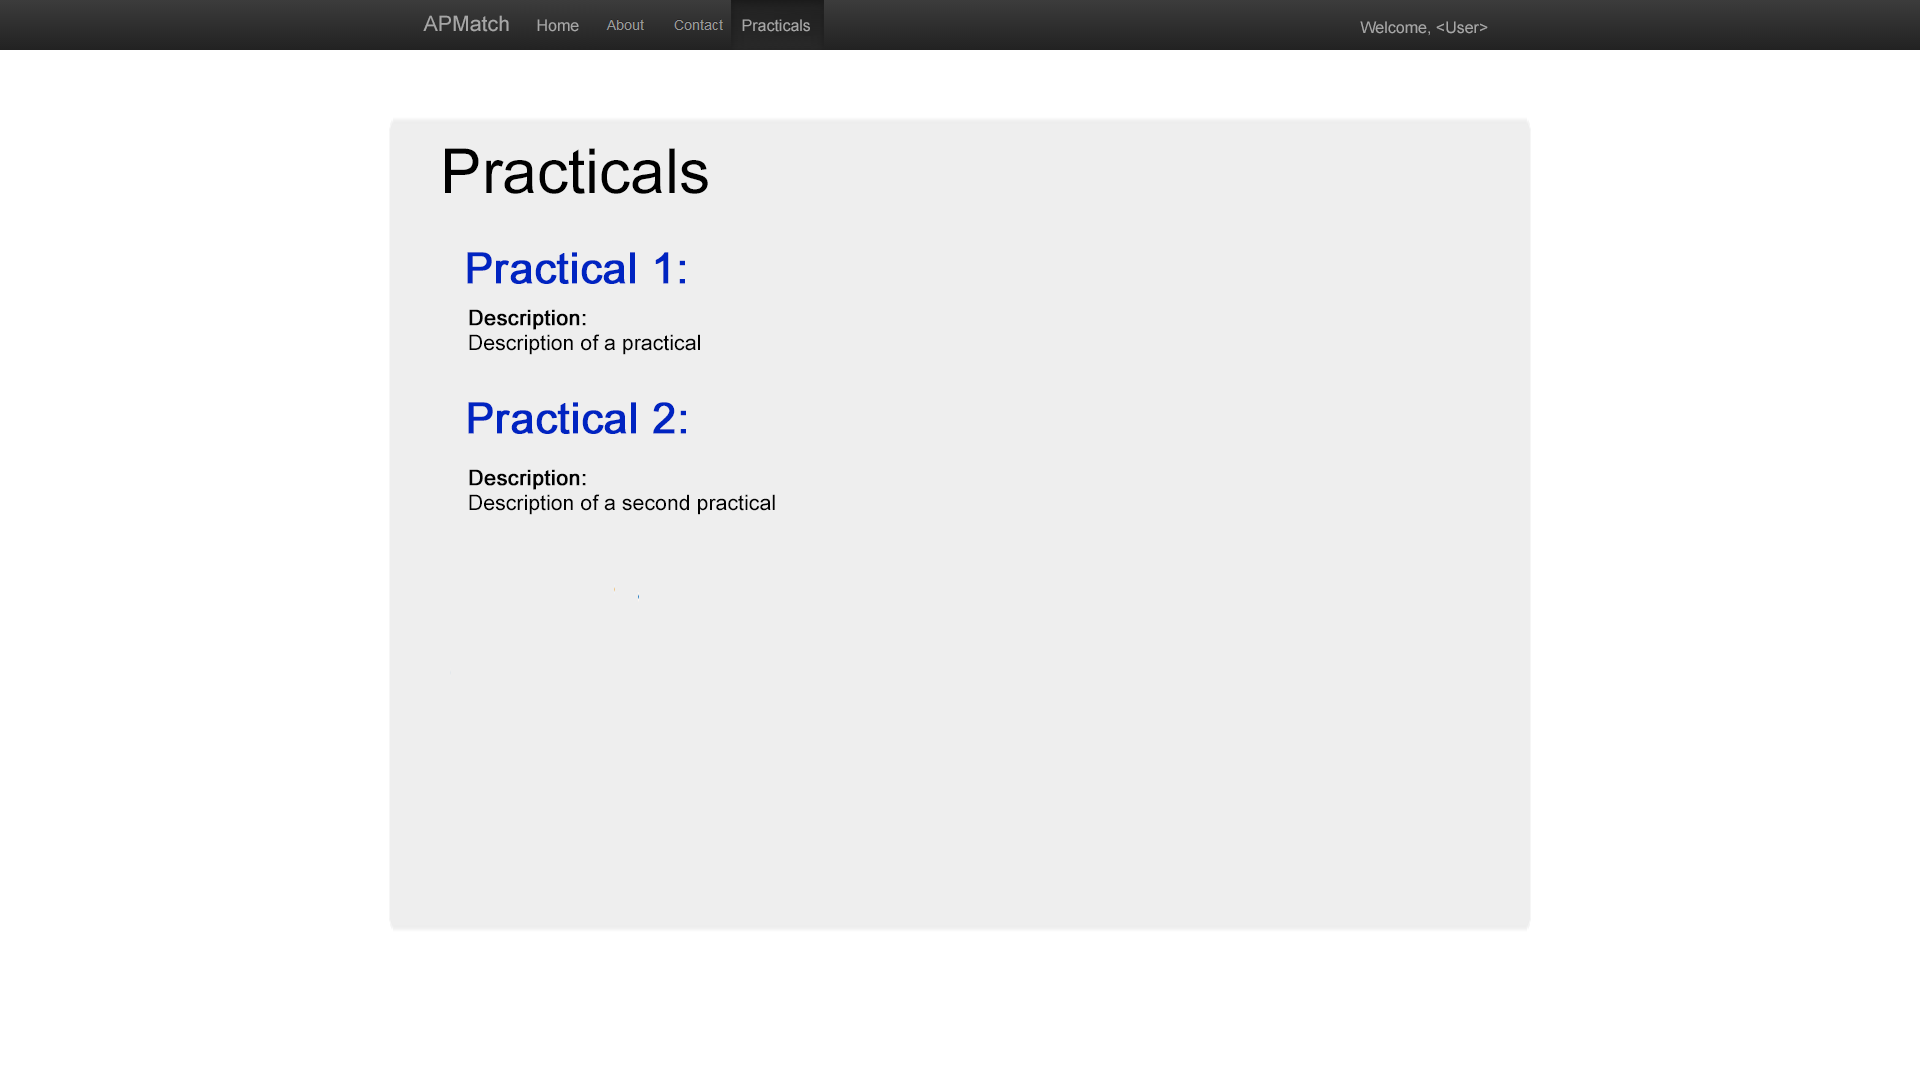
\includegraphics[width=\textwidth, frame]{images/mockup_practical_overview}
    \caption{Interface for the practical overview page}
    \label{mockup_practical_overview}
\end{figure}

\begin{figure}[H]
    \centering
    \captionsetup{justification=centering}
    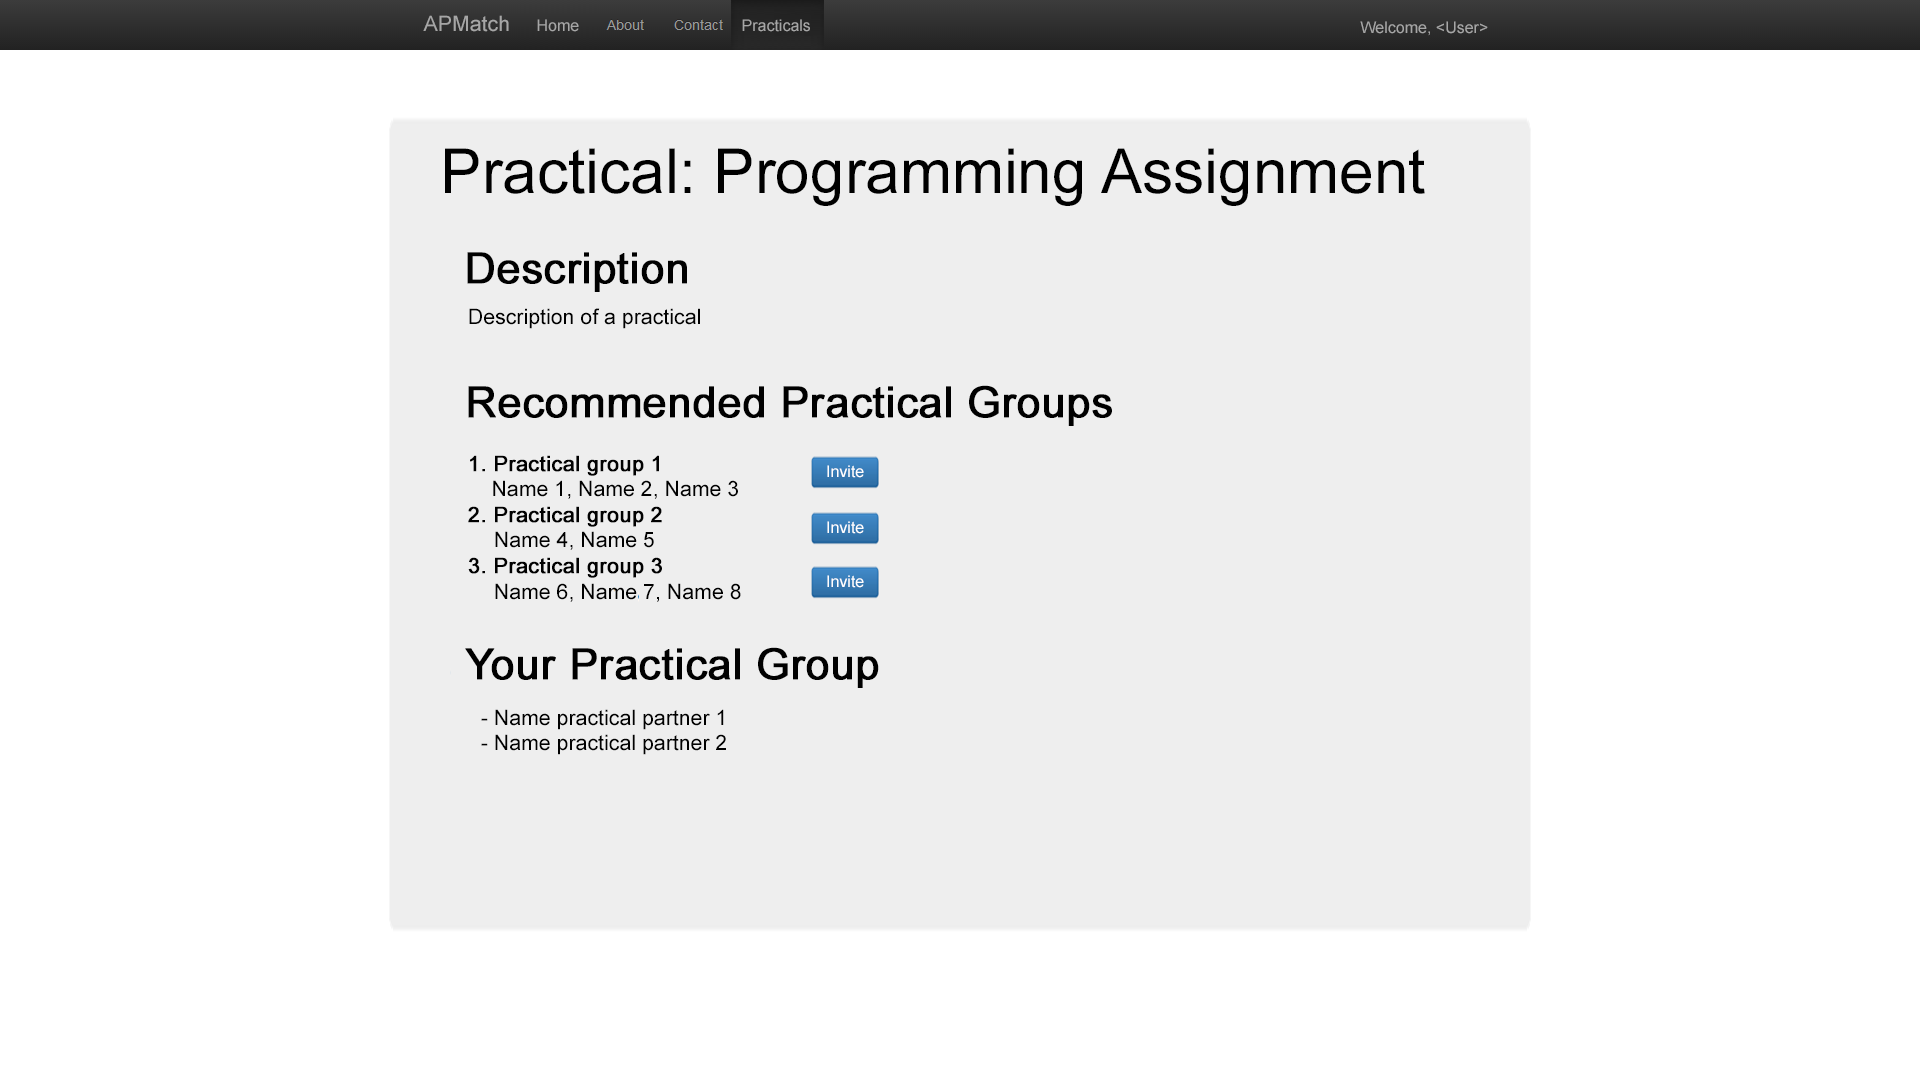
\includegraphics[width=\textwidth, frame]{images/mockup_practical}
    \caption{Interface for the practical page}
    \label{mockup_practical}
\end{figure}


\chapter{Project Methodology}
In this chapter we will describe the project methodology that we have applied to this project.
We will first divide the project into three phases.
For each phase we will specify the goal of this phase, the planning, the process strategy, the planned deliverables and the project roles.
Lastly, we define the tools that we have used during the project.
We have chosen for this particular form of documentation because in this way we can easily desribe the unique aspects of each phase.

\section{Global planning}
We have set up a global planning that splits up the project in phases.
Each of these phases has deliverables attached to them.
We will be mentioning our goals for each week.
Other important dates are also added to the planning.

\section{Phase 1}
\subsection{Goal}
The first phase aims to expand the knowledge of the group about the problem and it's requirements.
Secondly, it also gives time for the team members to analyse the problem for difficult subjects and to spend time finding a fitting solution.
Thirdly it gives the team members the time to set up the project infrastructure and to define the project methodology.
Lastly, the remaining time should be spend making a first start with the system design.

\subsection{Planning}
We planned phase 1 to be two weeks long.
With the first week having a focus on setting up the project and doing research to the problem and requirements.
The second week was more about defining the project methodology, analysing and researching the possible problems that we could encounter and making a first system design.
The second week was also used to finish up the research report.
\subsubsection{Planned deliverables}
At the end of phase 1 we wanted to have the following deliverables done:
\begin{itemize}
\item Research report
\item Plan of approach
\item First system design
\end{itemize}

\subsection{Process strategy}
During this phase we choose to not have a strict task distribution.
Many of the tasks at hand needed group thinking and group opinions.
For example, the interpretation of the problem description is something that can be thought out by a single person, but needs to be communicated about toward the other team members.
If not communicated enough, the resulting problem description may not be the same as how the team interpreted the client's description.
Things that needed to be done were documented in a spreadsheet.
In this way, every team member had insight into the things that still needed to be done.

\subsection{Project roles}
As said above, there was not a strict task distribution.
Following the advise of our group mentor, every week a different team member was the designated chairman and another team member was the designated secretary.
The chairman of the week had the responsibility to preside the weekly meetings and to maintain an overview of the tasks that were at hand.
The secretary had the responsibility of making minutes of both the weekly meetings and the meetings with the group mentors and client.
Next to these two roles, there were no other defined roles.

\subsection{Phase reflection}
%Nog te doen: schrijven over het verloop van deze phase

\section{Phase 2}
\subsection{Goal}
The purpose of the second phase was to provide a time frame in which both a basic system design can be made and the system design could be implemented.
During the second phase the roles were more strict since we wanted to follow a structured software development method.
This software development method is the framework known as scrum.
We will go into depth about this in the process strategy section.

\subsection{Planning}
We planned the second phase to be six weeks long.
The first week would be used to finish up the system design.
The other 5 weeks will be used to implement this system design.
During the final two weeks we looked into the user tests and the acceptance tests.
During this time there we also sent our source code to the Software Improvement Group for them to check.
The feedback that we got back will be 

\subsubsection{Planned deliverables}
During phase two we wanted to have the following deliverables done:
\begin{itemize}
\item Basic system design
\item User tests
\item Send the source code to SIG for the first review
\end{itemize}

\subsection{Process strategy}
During the implementation phase we used a known software development framework.
This development framework is known as scrum.
Scrum is based on the agile software development framework which can be used to 
manage software projects.
The time that we have to implement the system is limited so we did not have the time to research and design all aspects of the system. We need a software development framework that gave us the possibility to react to changes in requirements, but also to react to new insights given by our increasing understanding of the system as time progresses.
Scrum has a flexible approach to software development and satisfies the requirements that we have mentioned above.
In scrum, you only need a basic design of the system before you start implementing.
During implementation you provide daily feedback on your progress and the team can change the way things are programmed or have been programmed to steer the product in the proper direction.
We have defined the different roles associated with scrum (e.g. the product owner, development team, scrum master) as you can see below.

\subsection{Project roles}
The following table lists the different group members, their roles and a short description.
This description describes the role and responsibilities of the group member.\\
\begin{tabular}{|l|l|p{5cm}|}
\hline
Name & Roles & Description\\
\hline
Freek van Tienen & Lead Development & Responsible for implementation phase.\\
\hline
Floris Verburg & Scrum master and Quality Assurance & Responsible for the Scrum process, the quality of the code and test coverage.\\
\hline
Marijn Goedegebure & Project Manager and Reports & Manages the project and ensures that the requirements are met.\\
\hline
Leon Rothkrantz & Client, Group Mentor and Supervisor & Supervises the project, aides the group with difficulties and has issued the assignment.\\
\hline
Dragos Datcu &  Group Mentor and Supervisor & Supervises the project and aides the group with difficulties.\\
\hline
\end{tabular}
\subsection{Phase reflection}
%Nog te doen: schrijven over het verloop van deze phase

\section{Phase 3}
\subsection{Goal}
The goal of the third and last phase is to provide for time to finish up the project.
During this phase time has been reserved for finishing up the implementation, the final report and for the user tests.

\subsection{Planning}
During this phase there is time for completion of the implementation, finalization of the final report and creation of the presentation.
The completion of the implementation and the finalization of the final report will been done simultaneously.
The creation of the presentation will be done after the final report has been submitted.
After the final report is submitted we will also be looking into the feedback that we received from the SIG.
Three days before the presentation, the source code should be send to SIG for a final review.

\subsubsection{Planned deliverables}
During phase three we wanted to have the following deliverables done:
\begin{itemize}
\item Final report
\item Presentation
\item Improved implementation following the comments provided by SIG
\item Final review of SIG
\end{itemize}

\subsection{Process strategy}
The process strategy for this phase is completely equivalent to the first phase.

\subsection{Project roles}
The project roles for this phase are the same as for the first phase.

\subsection{Phase reflection}
%Todo, write a phase reflection

\section{Tools}
We have used several tools to support our development.
They helped us to maintain the quality of the code and improve the maintainability.
Some of these tools also helped with structuring the implementation phase.

\begin{itemize}
\item IntelliJ IDEA, is our Integrated Development Environment (IDE) which will facilitate the development and testing of our code.
IntelliJ will be integrated with the Play framework which will be helpful during development.
\item GitHub, is our on-line code and documentation repository.
It provides for a version control system, an issue tracker and code review possibilities.
We will be using it to store all our code and documentation's code (LaTeX).
\item Cloudbees
Cloudbees will be used to run our test environment, our continuous integration and the release environment.
It uses Jenkins for the continuous integration.
\item Play framework
The play framework gives us the possibility to easily create a web application using Java.
\item Findbugs is a plug in for Cloudbees and IntelliJ that gives us the possibility to let our java code be checked for small bugs using static analysis.
\item JaCoCo is a plug in for Cloudbees and IntelliJ that provides us with data analysis about our code coverage.
\item Checkstyle is a plug in for Cloudbees and IntelliJ that checks the code for coding standards.
This makes it ideal to enforce the coding standard for our project.
\end{itemize}


\chapter{System Design and Implementation}
\label{sec:design_implementation}

\section{Global System Design}
In this section we will explain how we designed the application and why we made several decisions.
We do this using different diagrams.
We have made for example a class diagram, a database diagram, sequence diagrams and state diagrams.

\subsection{Database}
In Figure~\ref{database_diagram}, our database diagram can be seen.
We will explain the structure of the database shortly.

\begin{figure}[h]
    \centering
    \captionsetup{justification=centering}
    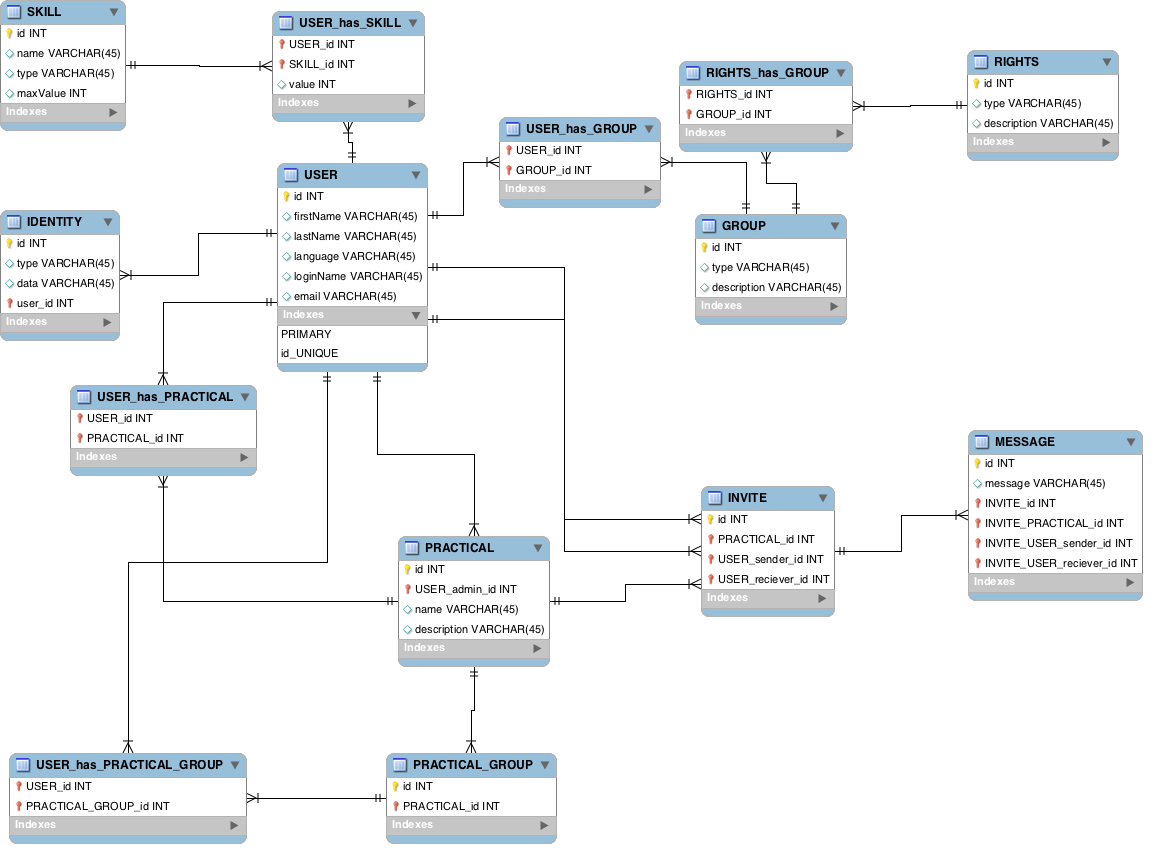
\includegraphics[width=\textwidth, frame]{images/database_diagram}
    \caption{The database diagram}
    \label{database_diagram}
\end{figure}

In the center of the diagram, the user is shown.
The user has a many to many relation with a group.
There are four different groups.
There is a group for students, for teachers, for administrators and one for guests.
It is obvious that a group can contain multiple users, but a user can also have multiple groups.
Users can be a teacher, as well as an administrator.

Every group has different rights.
The same right can also be assigned to multiple groups.
That is why we also have a many to many relation between a group and a right.

A user must also be able to log in.
To accomplish this, the user must have an identity.
An identity can only belong to one user.
If this should not be the case, the system would not be safe because other users have access to protected parts of the system.

A user can be part of multiple practical groups and a practical group consist of multiple users.
Therefore user and practical group also have a many to many relation.
This is the same for user and practical.

A practical group belongs to only one practical.
A practical can have multiple practical groups.
Therefore is this a many to one relation.

An invite has two many to one relations with a user.
An invite has a sender as well as an receiver.
There can only be one sender and one receiver for an invite.
But a user can send and receive multiple invites, therefore is this also a many to one relation.

Every invite belongs to only one practical.
These therefore also have a many to one relation.

The last relation is between an invite and a message.
These messages are for communication between the sender and the receiver of the invite.
An invite can have multiple messages and every message belongs to only one invite.

\subsection{Class Diagram}
In Figure~\ref{class_diagram} our application's class diagram can be seen.
This diagram is not complete with all the methods and attributes, but the most important methods and attributes are included.
For example, all the get and set methods are not included.

The structure of this diagram looks a lot like the database diagram.
In this diagram, we make a difference between a student and a user, because they can perform different actions.

For example, only a teacher can create courses.
A student cannot do this, a student can only sign up for this courses.

A student can also find possible group members.
These possible group members are determined by the recommender class.
With the getNextGroupMember method the next best practical partner will be calculated.
More about the matching algorithm can be read in Section~\ref{sec:algorithm}

The other methods are needless to explain.
The name of the methods tell the function.

\begin{figure}[H]
    \centering
    \captionsetup{justification=centering}
    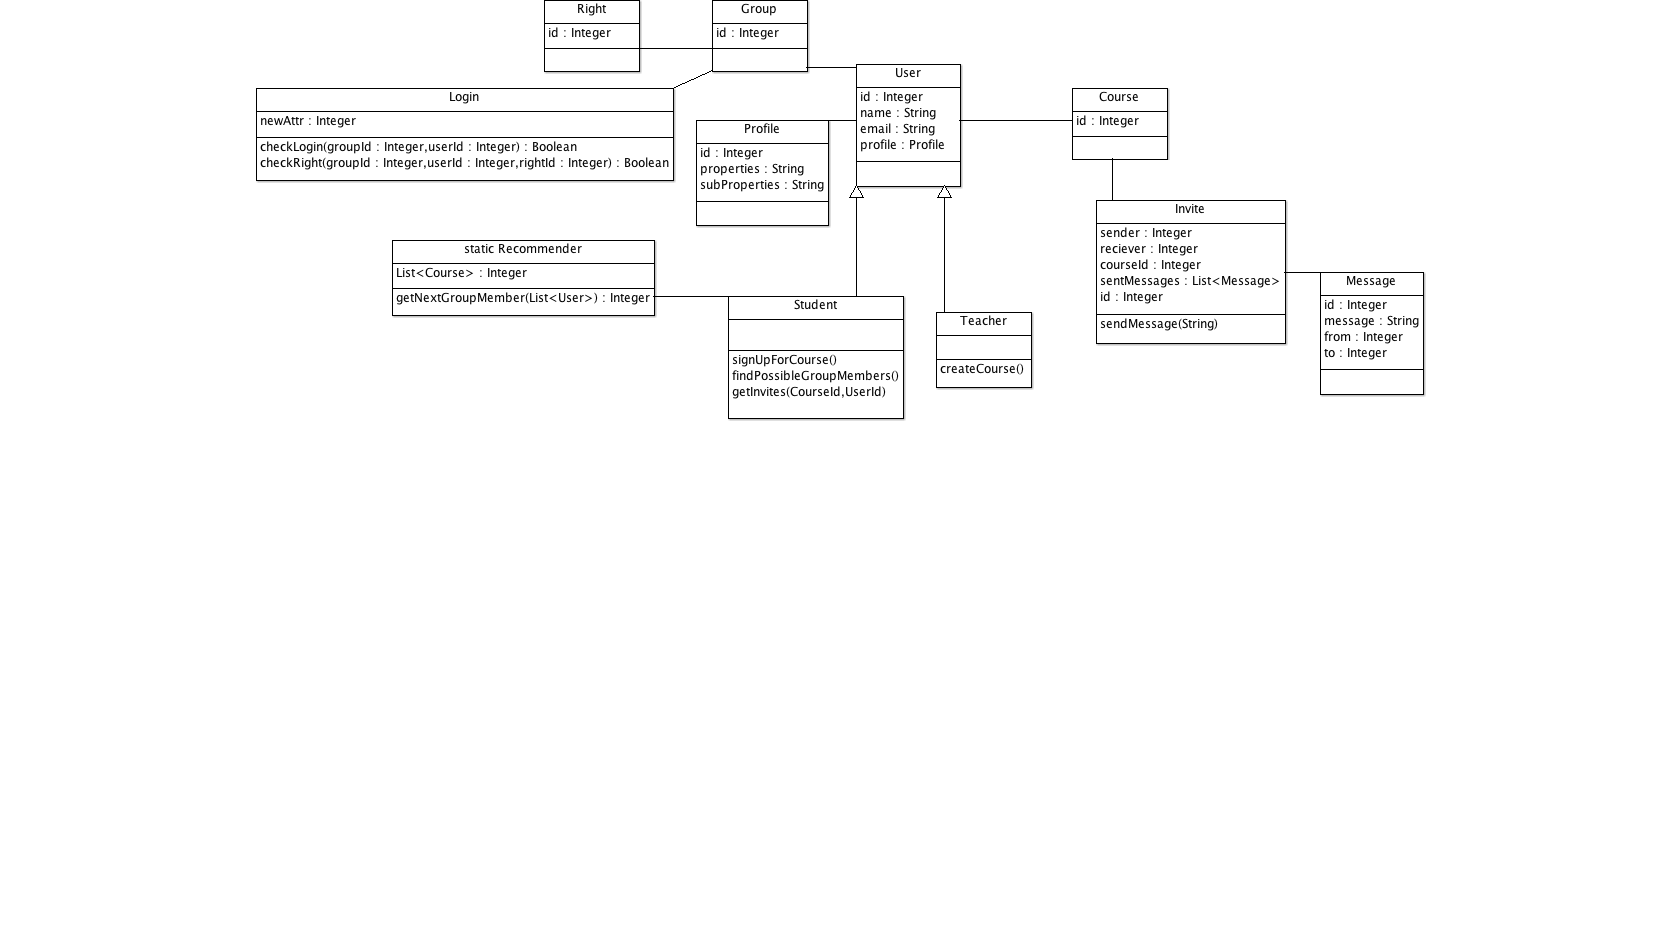
\includegraphics[width=\textwidth, frame]{images/class_diagram}
    \caption{The class diagram}
    \label{class_diagram}
\end{figure}

\subsection{State Diagrams}
In this section we describe the behaviour of our system with the help of state diagrams.
We describe this behaviour with two different state diagrams.
One diagram for the administrator and an other one for a student.

First of all, the administrator must be registered and logged in before he can perform any action.
When the administrator is logged in, he can create practicals.
When the practical is created, the administrator can edit and manage this practical.

One of the parts of managing the practical is managing the users that are enrolled for this practical.
The admin can remove users or even entire practical groups.

\begin{figure}[H]
    \centering
    \captionsetup{justification=centering}
    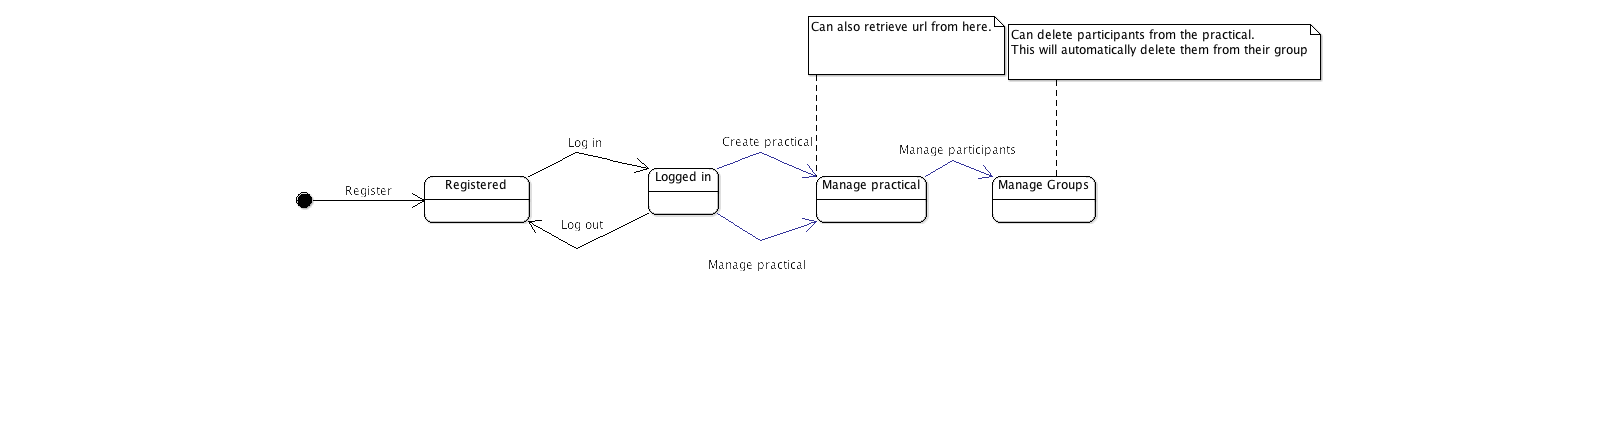
\includegraphics[width=\textwidth, frame]{images/state_diagram_admin}
    \caption{The administrator's state diagram}
    \label{state_diagram_admin}
\end{figure}

The student's state diagram is a little bit more complex.
The first part is the same as with the administrator.
The student also must be registered and logged in to perform any action.

When the student is logged in, he has two options.
He can either go to his profile, or manage his practical.
When he chooses to go to his profile, he can view or edit it.

The courses have some more options.
First of all, the student can see which fellow students are recommended to join his group.
The student can invite these students to join his practical group.

The student can also view the overview of his invites.
This overview includes both received and sent invites.
When the student accepts an invite, both the practical groups are joined.

\begin{figure}[H]
    \centering
    \captionsetup{justification=centering}
    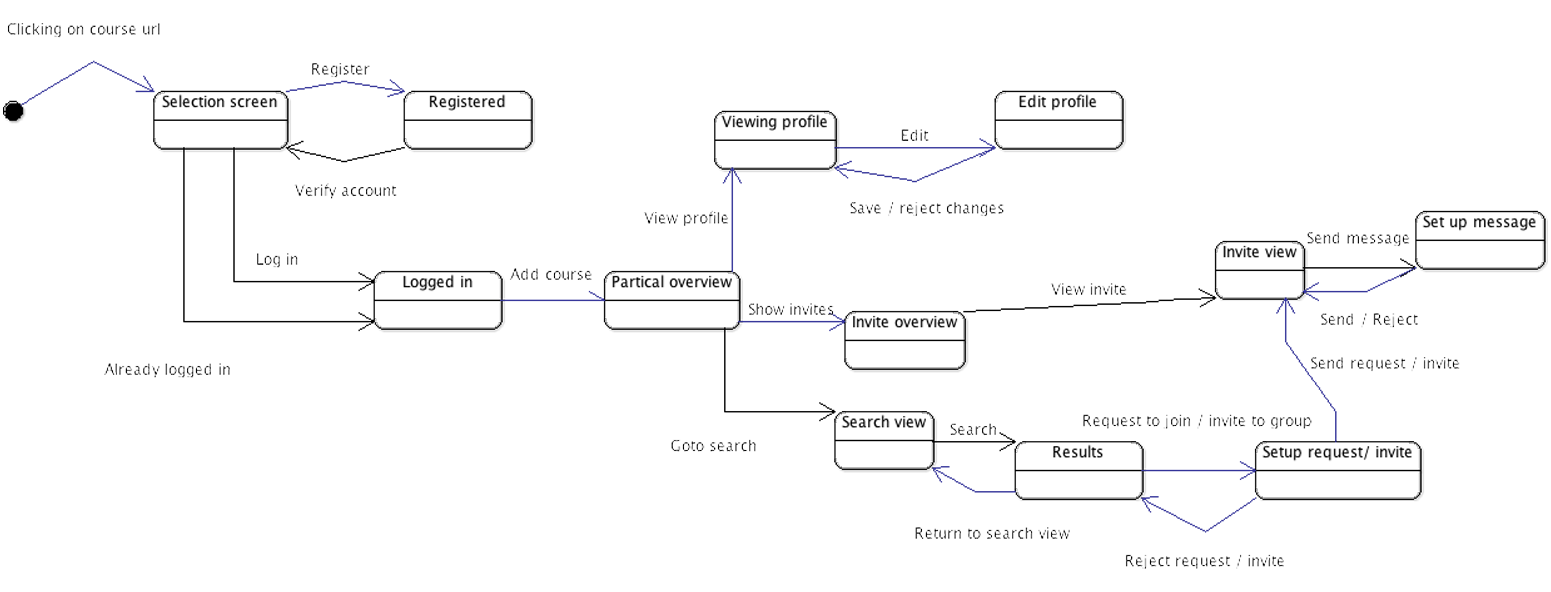
\includegraphics[width=\textwidth, frame]{images/state_diagram_participant}
    \caption{The participant's state diagram}
    \label{state_diagram_participant}
\end{figure}

\subsection{Sequence Diagrams}
In this section we explain the sequence diagrams.
We have only made a sequence diagram for logging in, but because of the Model View Controller structure (Section~\ref{sec:mvc}) most of the actions have a similar sequence diagram.

The user only has direct contact with the views.
The views send the information that the user provided to the controllers.
After that, the controllers collect the required information from the database via the models.

When the controllers have all the required information, they execute their calculations.
After the calculations are fully executed, the results will be sent back to the views.
The views display these results and via these views the results will reach the users.

\begin{figure}[H]
    \centering
    \captionsetup{justification=centering}
    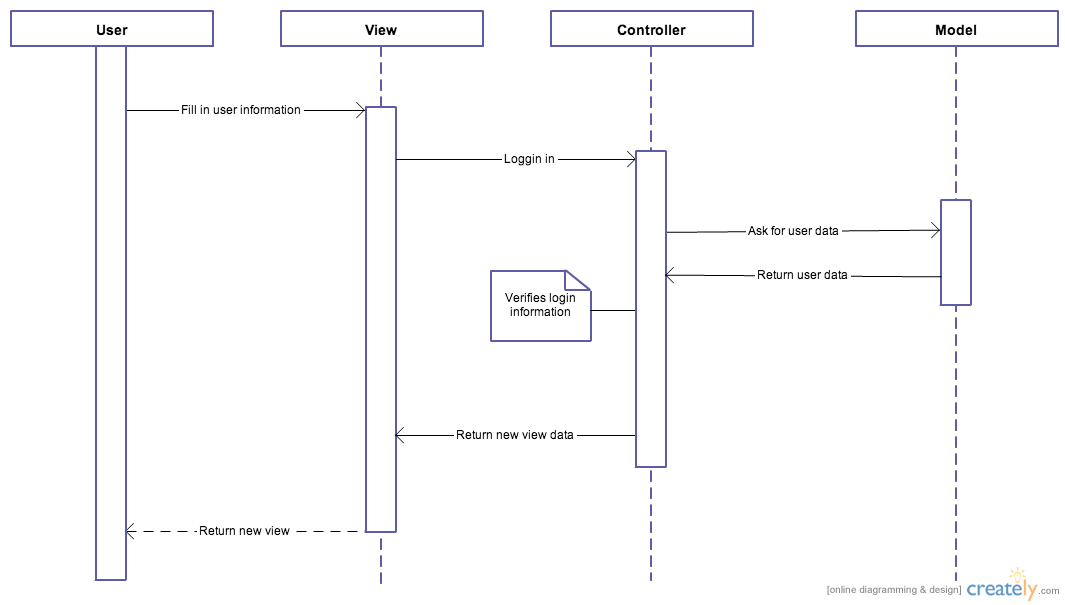
\includegraphics[width=\textwidth, frame]{images/sequence_login}
    \caption{The sequence diagram for logging in}
    \label{sequence_login}
\end{figure}

\section{Graphical User Interface Mockups}
We have multiple important features in our application.
Each of these features has an own graphical user interface (GUI).
Below, we will provide mockups from the graphical user interfaces of the most important features.

\subsection{Profile}
As can be seen in Figure~\ref{mockup_profile}, a user can view someone's (or it's own) profile.
The user can see the basic profile information which the user has filled in himself.

If a user is looking for a practical partner, he can get a better impression of that person when he gets an overview of the profile information of that person.
This is just a simple page, because the user should quickly get an impression of the student.\\

\begin{figure}[H]
    \centering
    \captionsetup{justification=centering}
    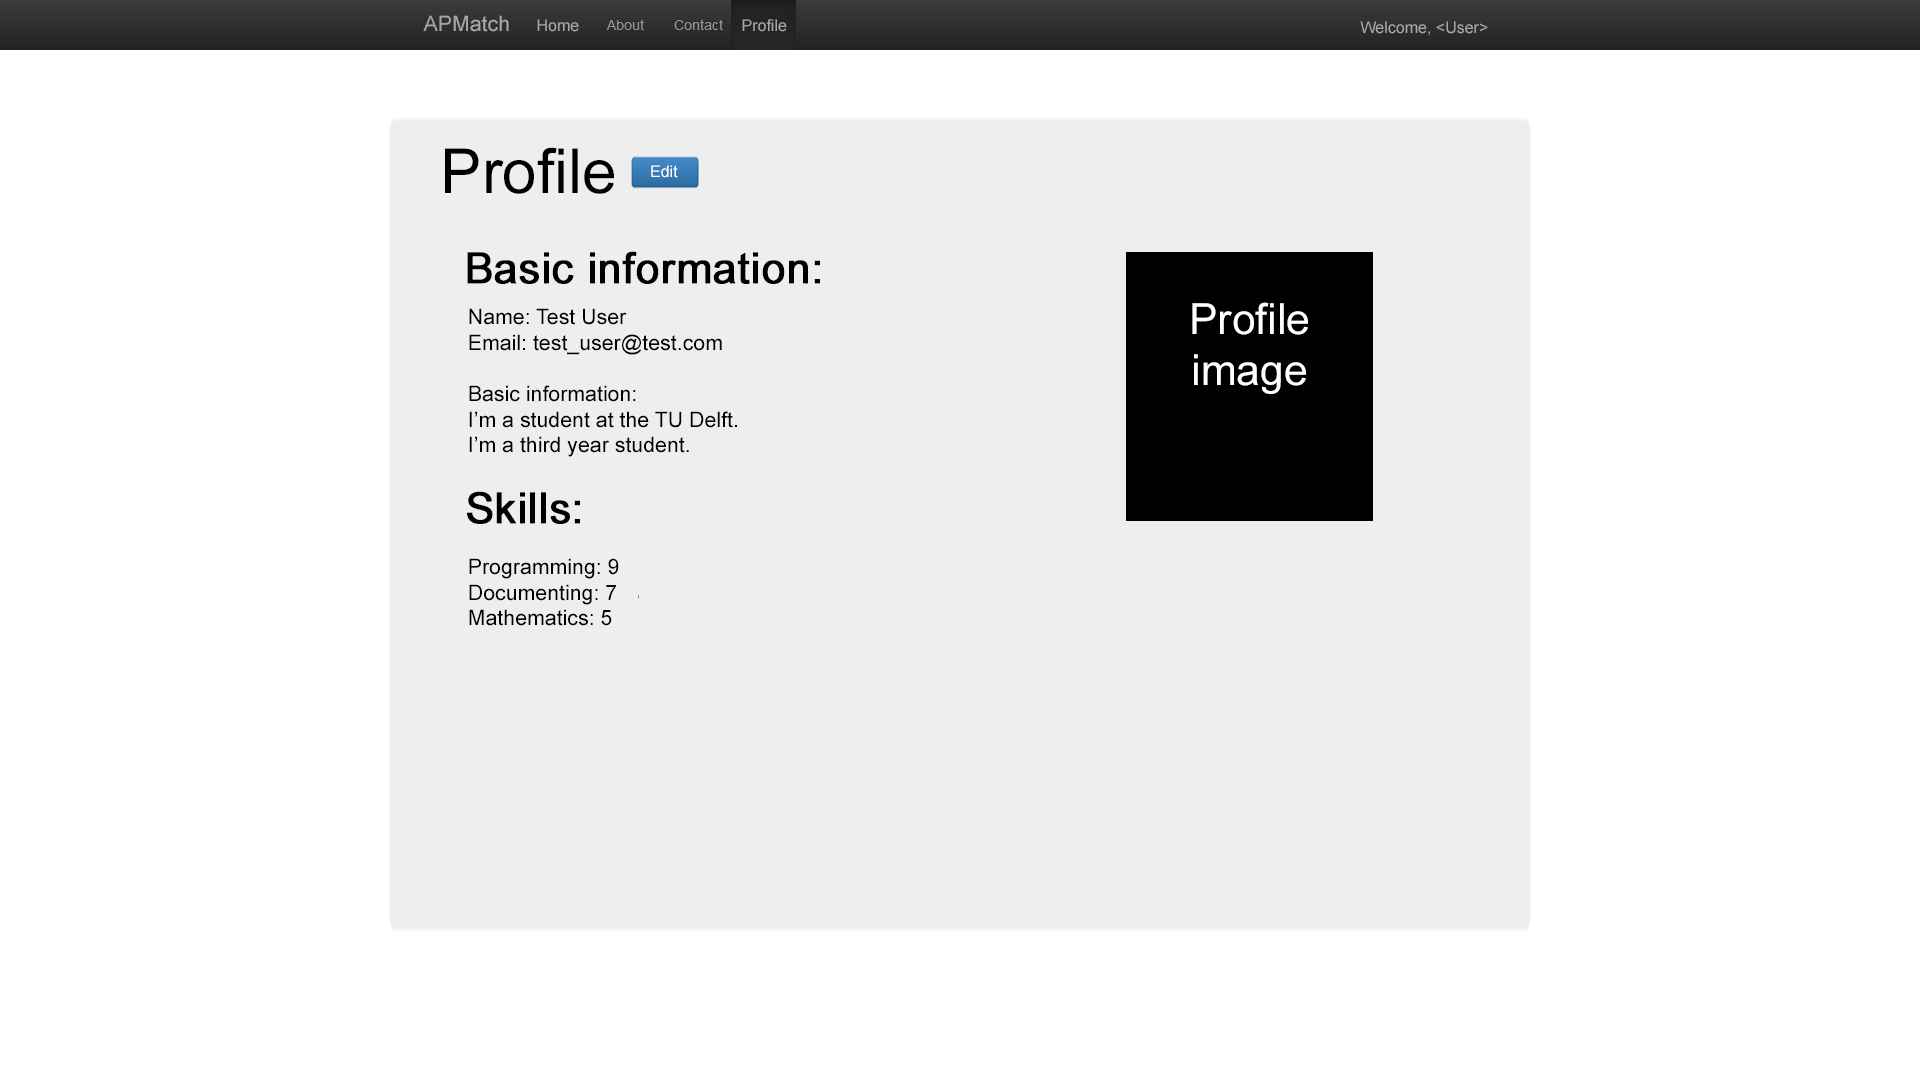
\includegraphics[width=\textwidth, frame]{images/mockup_profile}
    \caption{Interface for the profile page}
    \label{mockup_profile}
\end{figure}

In Figure~\ref{mockup_edit_profile}, the page for editing the profile can be seen.
On this page, the user can edit his basic profile information as well as the level of his skills.
He can also change his password and his profile image.
This information will be taken into account while determining the recommended practical partners.
So it is important for the users to be able to fill in this information easily.

\begin{figure}[H]
    \centering
    \captionsetup{justification=centering}
    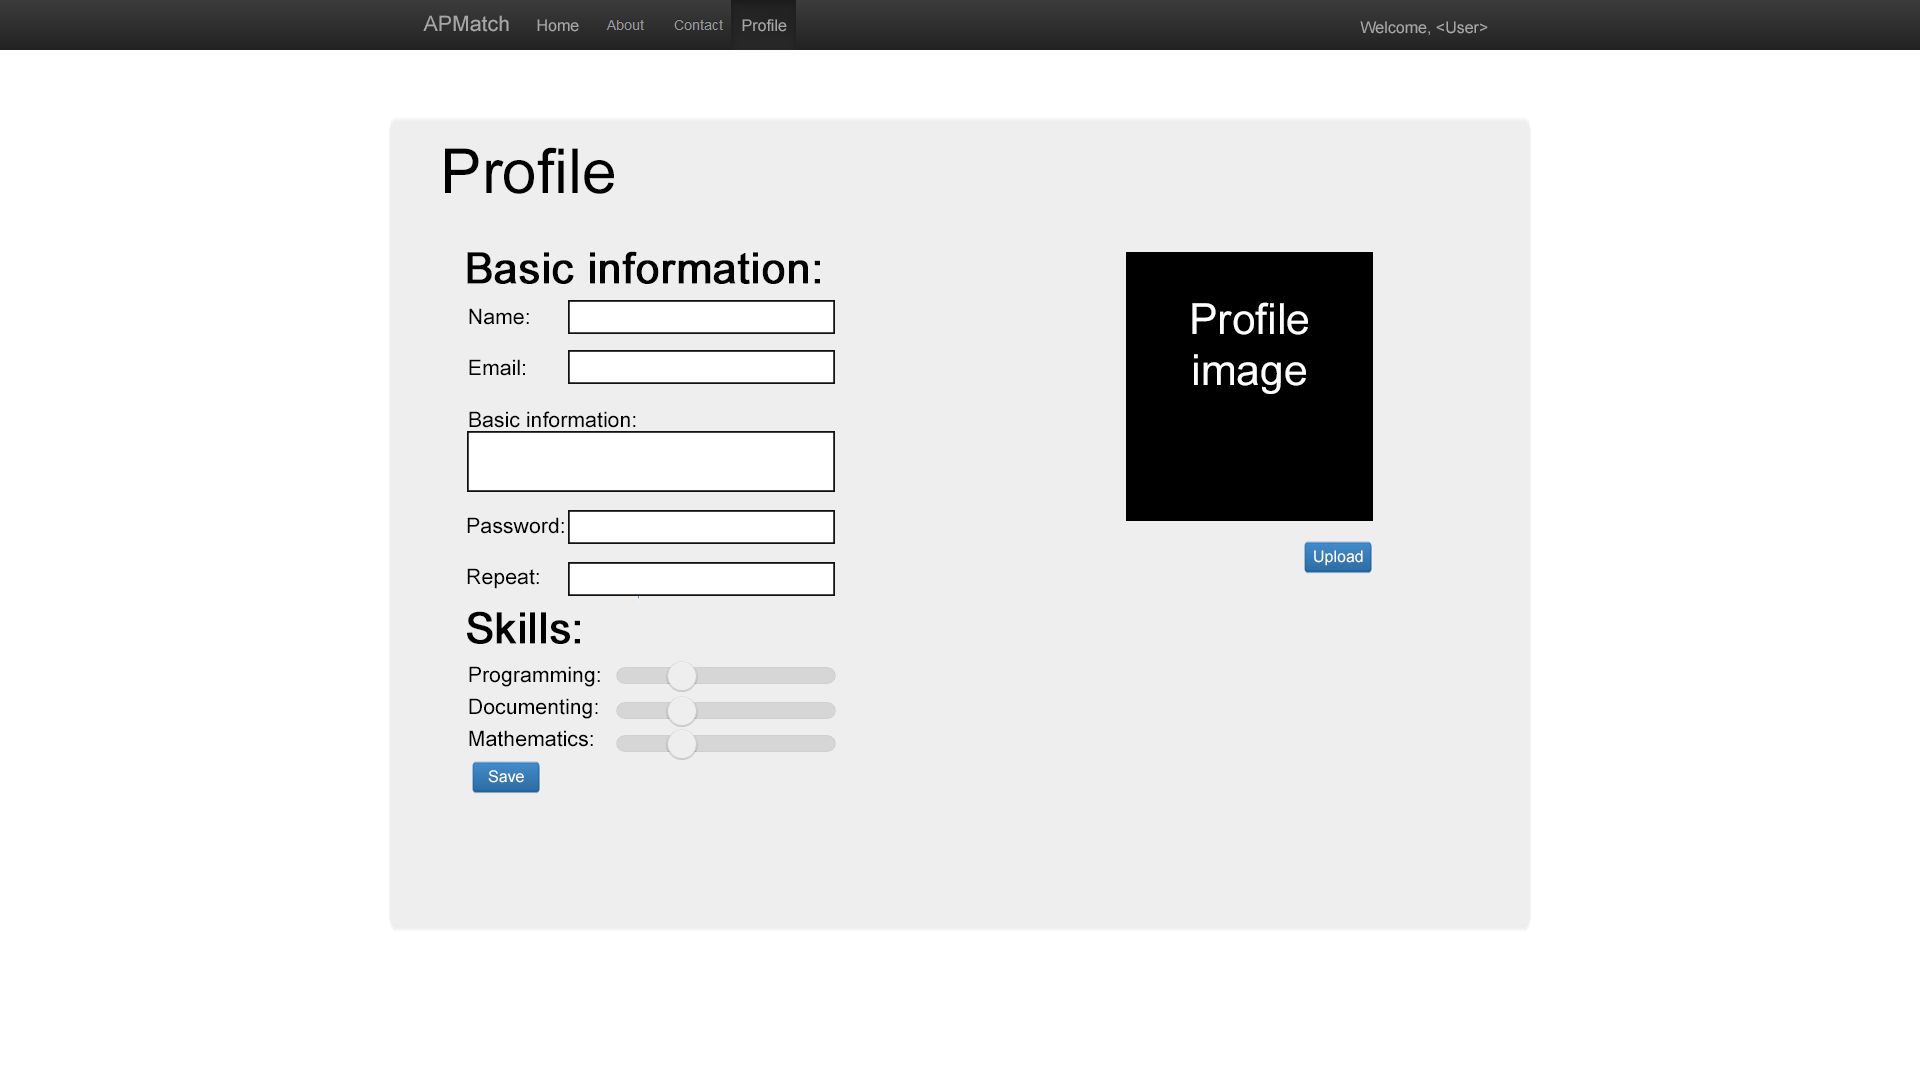
\includegraphics[width=\textwidth, frame]{images/mockup_edit_profile}
    \caption{Interface for editing the profile}
    \label{mockup_edit_profile}
\end{figure}

\subsection{Practical}
The main feature in our application is recommending practical partners.
Therefore the users need to be able to register for a practical assignment.
The user receives a link from the teacher and when they have clicked on it, the user is registered to the practical.
The practical is then added to the user's practical overview.
Such an overview can be seen in Figure~\ref{mockup_practical_overview}

\begin{figure}[H]
    \centering
    \captionsetup{justification=centering}
    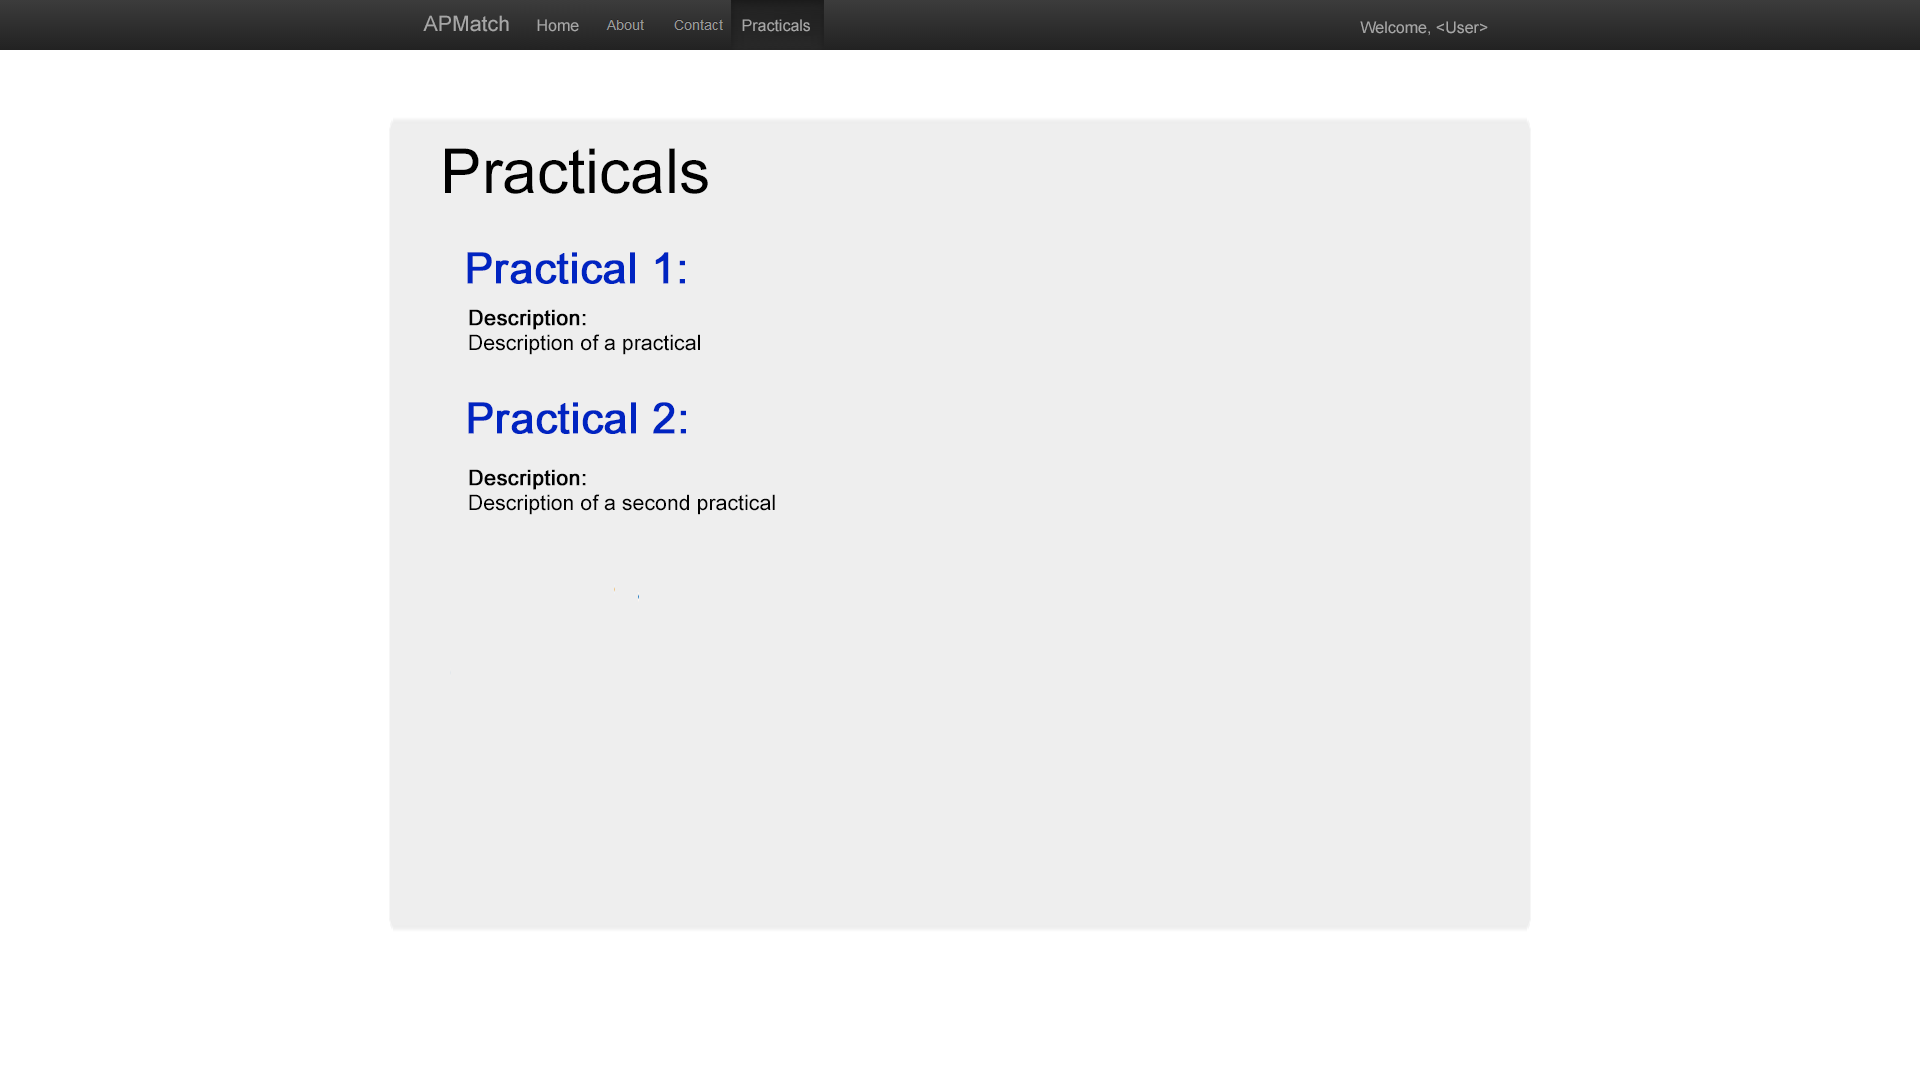
\includegraphics[width=\textwidth, frame]{images/mockup_practical_overview}
    \caption{Interface for the practical overview page}
    \label{mockup_practical_overview}
\end{figure}

In Figure~\ref{mockup_practical}, the user can see a page for a certain practical.
First of all, there is some information about the practical itself.
We show a short description of the practical.

After that, we show the most important part, the recommendation.
The application determines which other practical groups matches the user's group the best.
On this page the user can click on the practical group for more information.
The user can also invite a practical group to join his practical group.

After the recommendation part, we also show the user's current practical group.

\begin{figure}[H]
    \centering
    \captionsetup{justification=centering}
    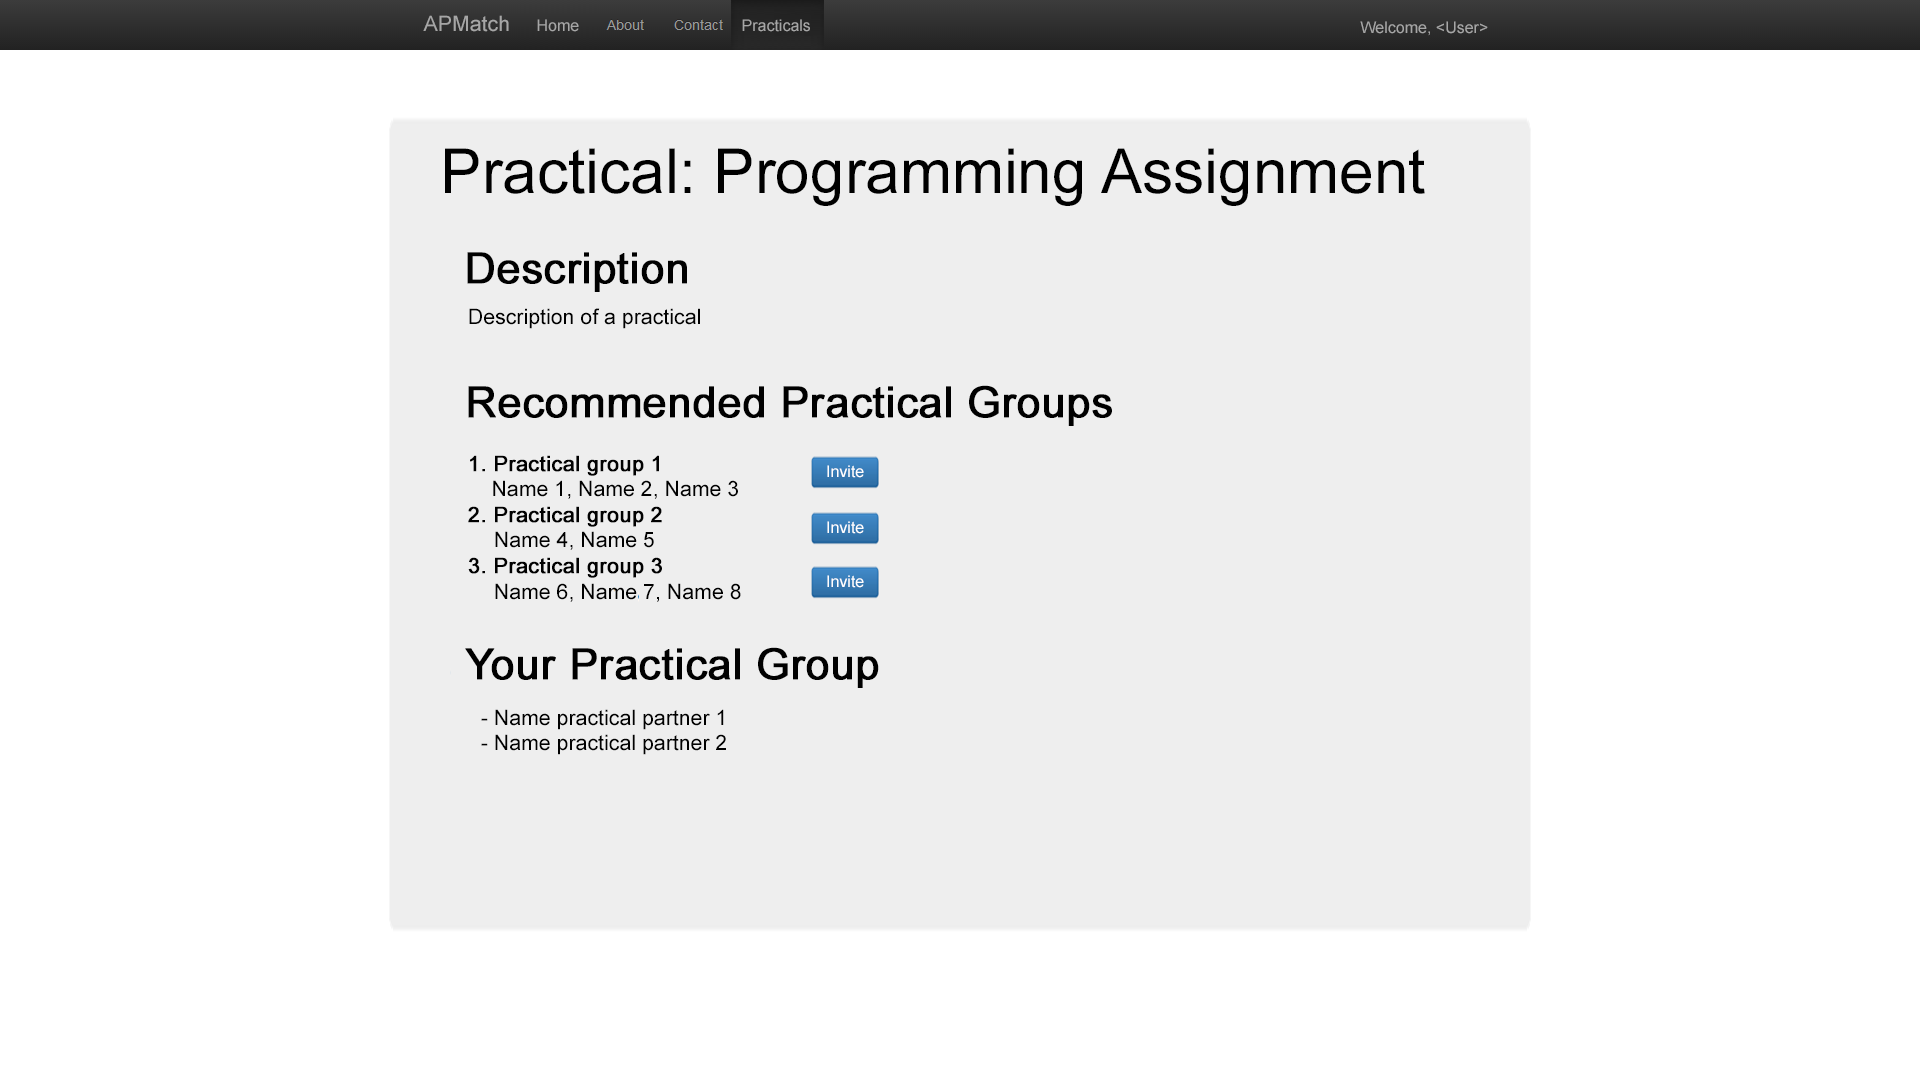
\includegraphics[width=\textwidth, frame]{images/mockup_practical}
    \caption{Interface for the practical page}
    \label{mockup_practical}
\end{figure}

\section{Model View Controller}
\label{sec:mvc}
As mentioned earlier, we are using the Play Framework. 
This frameworks follows the Model View Controller (MVC) architectural pattern applied to the Web architecture\cite{playframework_mvc}.
This pattern splits the application into separate layers: the Presentation layer and the Model layer. 
The Presentation layer is further split into a View and a Controller layer.

\subsection{Controller}
The \textbf{Controller} responds to events (typically user actions) and processes them, and may also invoke changes on the model.
In a Web application, events are typically HTTP requests: a Controller listens for HTTP requests, extracts relevant data from the 'event', such as query string parameters, request headers... 
And applies changes on the underlying model objects.

In Play, a Controller is a Java class where each public, static, method is an \textbf{action}.
An action is a Java entry point invoked when a HTTP Request is received.
The Java code from the Controller class is not really object oriented: it is mainly procedural code.
The action method extracts relevant data from the HTTP request, reads or updates the model objects, and sends back a result which is wrapped into an HTTP Response.

\subsection{Model}
The \textbf{Model} is the domain-specific representation of the information on which the application operates.
Domain logic adds 'meaning' to raw data (e.g., calculating if today is the user's birthday, or the totals, taxes, and shipping charges for a shopping cart).
 Most applications use a persistent storage mechanism such as a database to store data.
MVC does not specifically mention the data access layer because it is understood to be underneath, or encapsulated by, the Model.

In Play, the domain model object layer is a set a Java classes using all the object oriented features available from the Java language. 
It contains data structures and operations on which the application operates. 
Whenever model objects need to be saved into a persistent storage, they may contain some glue artefacts like JPA annotations or SQL statements.

\subsection{View}
The \textbf{View} renders the model into a form suitable for interactions, typically a user interface.
Multiple views can exist for a single model, for different purposes.
In a Web application the view is usually rendered in a 'Web format' like HTML, XML or JSON.
However there are some cases where the view can be expressed in a binary form, e.g. dynamically rendered chart diagrams.

In Play, most of the application views are generated using an efficient template system provided by play. 
The Controller gets some interesting data from the model layer, and then applies a template to decorate these objects. 
This packages contains HTML, XML, JSON and other template files with special directives used to dynamically generate the model representation.
\\
\begin{figure}[h]
  \centering
    \captionsetup{justification=centering}
    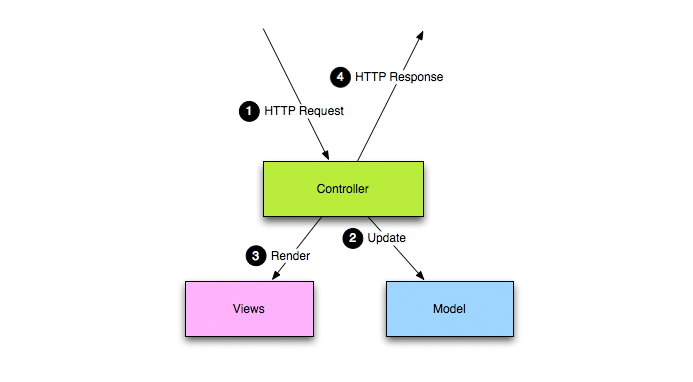
\includegraphics[width=\textwidth]{play_mvc}
    \caption{Play Framework MVC structure}
  \label{play_mvc_image}
\end{figure}


\section{Implementation}
In this section we will describe the software implementation of APMatch.
We will start of with a global implementation description of our APMatch system and then we will continue with some more advanced topics.

We chose to explain some more about both the invites and the matching algorithm.
For the invites we explain what our difficulties were and which situations were hard to implement, while for the matching algorithm we will explain some more on how it works and why we chose it.

\subsection{Global}
During the implementation we chose for the git feature workflow as described in section \ref{software_development_method}.
Most of the time this leads us to small and nice feature's which added both the model as well as the visuals to the APMatch system.
There were some exceptions like the Invites and Matching algorithm which were a lot harder to implement than expected.
These big feature's sometimes broke our workflow, because there were too many dependencies between the different features.
Luckily most of the time there were enough other feature's that could be implemented to solve the issue of waiting on the dependencies to be implemented.

Our global implementation went as planned and made use of the MVC design method of the Play Framework.
This lead to a nice structured way of models that related closely to the database model, containing most of the functionality of the APMatch system.
We also extended the MVC model a bit with a helper package which contains functionalities like hashing, Linkedin and the matching algorithm.
The helper classes don't relate to the database model, but will supply the needed functionalities for the controllers.

The controllers of the of the MVC model were defined in six different controllers: Application, Authentication, Invite, Practical, PracticalGroup and Profile.
The Application controller only provides the static pages like the home page, contact page and the information page.
The Authentication controller provides the functionalities for both the Linkedin login, and the normal authentication and registration.
All the other controllers provide the functionality for all the pages which relate to the subjects of their name.

\subsection{Invites}
One of the most underestimated parts of the implementation of APMatch was the invites system.
This part took by far the most time during the implementation phase, but was at first estimated as a part which could be quickly implemented.
This underestimation was mostly caused by the complexity of the invites system, which we will explain in the following paragraphs.
After that we will explain how we solved this difficult invite system, and conclude with what could be improved to make it even better.

So why is this invite system so complex?
This all is mainly caused by the problem that occurs when creating practical groups larger than two.
Creating a group larger than two requires either a group manager to create and maintain invites, or a different way of inviting people when the user is joined in a practical group.
This is needed because of the fact that having the possibility for all the group members to invite other people could lead to several conflicting situations.
So the easiest way to solve this is by creating a group manager, which would be the only user that has the rights to send and invite other users.

But then how do we choose a group manager?
We could of course easily solve this by doing it random, but that could lead to strange situations and then group manager functionalities also need to be added, to for example change the group manager.
To avoid these situations we then chose to instead of doing it random, make the inviter that forms the group the group manager.
This will make it sure that when the user accepts a certain invite he also knows who will be the group manager and also can depend his choice on that.

Despite the fact that we now solved both the complex system of having more then two group members, there were still other problems that also caused our underestimation.
This was due the fact that the user could have multiple open invites available at a certain time, both send invites and received invites.
Here we could have chosen to deny the user to have multiple outstanding invites to users, but because we expect that there will be a lot of inactive users this seems very implausible.
Users will then have to wait a certain amount of time for an inactive user, while other possible groups members might join other groups.
This is why we chose to implement it that when an invite is accepted and the user is not becoming a group manager, all the other invites will be rejected.
Hereby the problem of having multiple open invites at a certain time is solved.

One of the last problems we found during the implementation of the invites system was the fact that the user should be able to invite a group.
This caused two different subproblems, one person inviting a group and a group inviting another group.
Both were dealt with in the same way, by defining that a single person is also a group with just one person in it.
This only left us with the merging of two groups which was done the same way as joining one by one.

Because of all these all these edge cases we needed to test the invite system very carefully using a lot of unit tests.
Finding these edge cases, defining the edge cases and then writing the unit tests for these edge took more time than expected.
Initially we didn't taught of all these edge cases and were just thinking of a simple invite system.

For the future we advise to first think out the whole invite system and split it up in smaller features.
Then both the progress will be easier to track and writing tests cases will also be easier.
We also advise to make it more understandable for the user what exactly is happening during the invites.
This means that the users needs to know what happens to his other invites when he for example accepts an invite.
Also hiding the fact that the user is in a practical group on its own should make it more understandable for the user what is happening with the invites.

\subsection{Matching algorithm}
\label{sec:algorithm}
For our matching algorithm we used our custom designed algorithm.
This algorithm uses the skills defined by the user and the teacher to find the best matching with the preferences of the teacher.
We will first give a description of the algorithm followed by a formal description.
After that we will give a description about the complexity and will conclude this section with why we chose this implementation.

Before we start explaining the algorithm we will first describe how to calculate the distance for a certain practical group.
Calculating the distance of a practical group is done by going through the skills defined by the practical teacher.
We will then calculate the average of the values of the skills of all the users in the practical group and the users' practical group combined.
Then all the averages are multiplied with each other and then the root of the amount of skills in the practical is taken.
This resulting number will be defined as the distance.

The matching algorithm starts with a practical and user.
It will start with going through the different practical groups in the practical.
To simplify the algorithm we chose to make sure every user is in a practical group.
This means that when an user doesn't have any practical partners he is still in a practical group with only himself in it.
While going trough the different practical groups it will calculate the distance as described in the previous paragraph.
After calculating the distance with every other practical group and saving this in a map, this result is sorted by descending distance.
Then we start recommending practical groups to the user starting by the top of the list.
The formal definition of this algorithm is visible in Figure \ref{recommend}.

\begin{figure}[H]
 \centering
\begin{algorithmic}
\Function{Recommend}{$practical$, $user$}
	\State $resultList\gets$ Empty map of PracticalGroup and distance
	\ForAll{$practicalGroups$ in the $practical$}
		\State $distance\gets 0$
		\ForAll{$skills$ in the $practical$}
			\State $average\gets 0$
			\ForAll{$users$ in the $practical$}
				\State $average\gets average + SkillValue(user, skill)$
			\EndFor
			\ForAll{$users$ in the $user$ practical group}
				\State $average\gets average + SkillValue(user, skill)$
			\EndFor
			\State $average\gets average / (amount\_of\_users)$\Comment{The amount of users in the practical}
			\State $distance\gets distance * (average - SkillValue(Practical, Skill))$
		\EndFor
		\State $distance\gets distance ^ {(1 / amount\_of\_skills)}$\Comment{The amount of skills in the practical}
		\State $resultList\gets resultList + (practicalGroup, distance)$
	\EndFor
	\State Sort the $resultList$ by descending $distance$
	\State \textbf{return} $resultList$
\EndFunction
\caption{The recommendation algorithm}\label{recommend}
\end{algorithmic}
\end{figure}

To Analyse the complexity we need the following measurements.
We define $n$ as the amount of practical groups in a practical.
We define $m$ as the amount of skills defined in a practical.
We define $j$ as the amount of users in a certain practical group plus the amount of users in the user's own practical group.
Since in the first loop we go trough the practical groups to calculate the distance we start with a time complexity of $O(n)$.
Inside this loop we go trough each of the skills defined in the practical to calculate the average which will give us $O(n*m)$.
In order to calculate this average we need to go trough all the users in our practical group and the practical group examined.
This will lead to a time complexity of $O(n*m*j)$.
As one of the last steps we still need to sort the list of the practical groups which will be done in a time complexity of $O(n*log(n))$.
All this combined will lead into a total time complexity of $O(nmj+n*log(n))$ which for small $m$ and $j$ will lead to a total time complexity of $O(n*log(n))$.

We chose this implementation, because it is very easy to understand and very adjustable implementation of the algorithm.
There are several ways to optimise the algorithm by using precomputing.
This can be done for example during the defining of the skills by the user and will save execution time when viewing recommended solutions.
Next to that we have shown in the previous paragraph that with both a small amount of skills defined by a practical and with a small amount of users in practical groups, this algorithm will run in $O(n*log(n))$.
Since this will be the case, because both sizes are limited this will be fast enough to run while recommending without precomputing.
All these cases prove that the algorithm is good enough for recommendation system.





\chapter{Testing}
In this chapter we will be talking about the different techniques that we have employed to test the different aspects of the system.
We will first be talking about the different kind of unit tests that we have written.
These tests provide for a basic code coverage.
After this we will be talking about what kind integration tests we have performed to ensure the connection between the different components.
Lastly we will be talking about the acceptance tests that were performed.

\section{Testing methods during the implementation phase}
\subsection{Unit testing}
During the implementation phase a feature is only complete when it is fully tested.
This is done by running the system and testing it by the programmer, but also done by running automated tests.
These automated tests are required for achieving a good code coverage and for ensuring the code to work appropriately.
The tests that are written for other features will be always run after the feature has been merged.
This ensures that other features that may change the working of the code does not let the tests fail.
So all the features that were already in the system will still work even after the merging of the new feature.

In figure~\ref{testresulttrenddev} you can see the increasing amount of tests that increase with each pull request that has been merged with the development branch.
\begin{figure}[h]
    \centering
    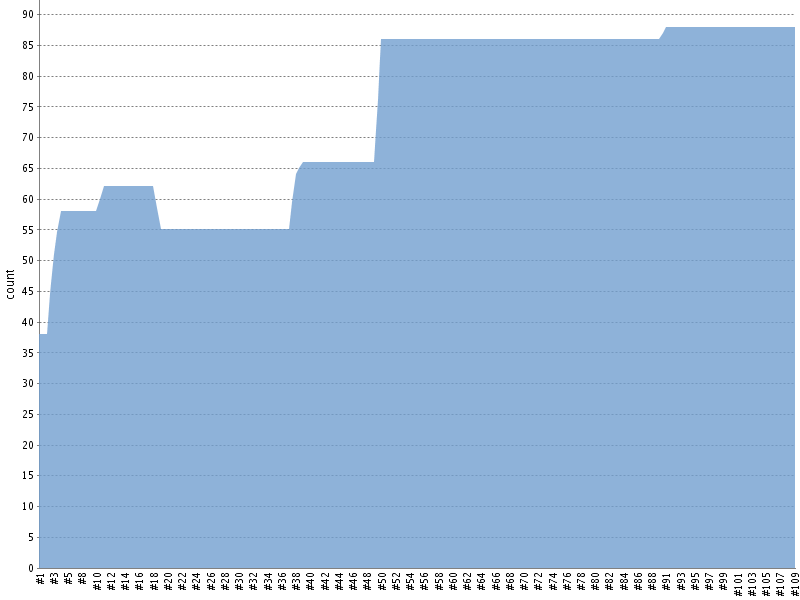
\includegraphics[width=\textwidth]{images/TestresultTrendDev2}
    \caption{Amount of tests per build}
    \label{testresulttrenddev}
\end{figure}

In figure~\ref{testresulttrendpullrequest} you can see the increasing amount of tests of the different pull requests that have been made.
In this image you can clearly see that when sometimes when a new feature is added, some tests start to fail.
Due to our continuous integration we could spot the errors early and make sure that they are fixed before merging with the development branch.

\begin{figure}[h]
    \centering
    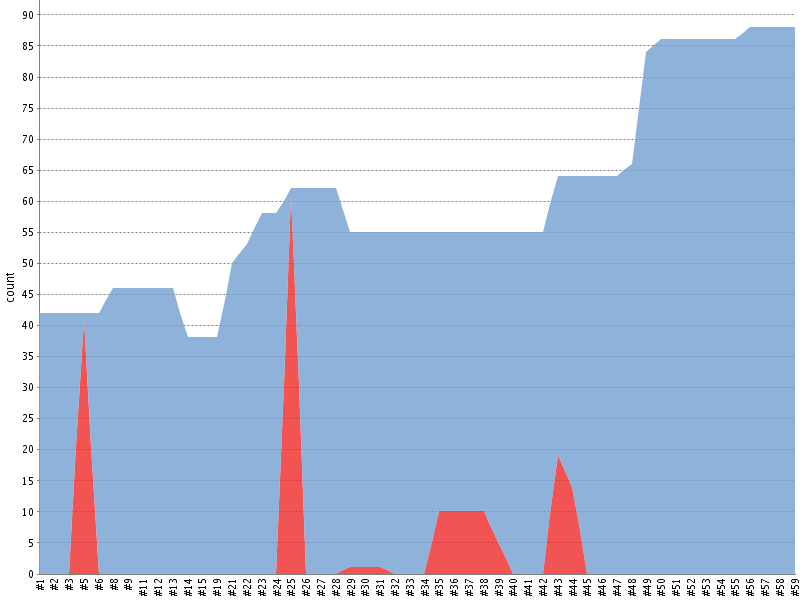
\includegraphics[width=\textwidth]{images/TestresultTrendPullRequests}
    \caption{Amount of tests per build of a pull request}
    \label{testresulttrendpullrequest}
\end{figure}

Figure~\ref{testresulttrendpullrequest} shows how not every pull request is without errors.
All of these errors first had to be resolved before the pull request could be merged.\\

Figure~\ref{codecoveragetrenddev} depicts the code coverage achieved by the tests.
The goal is to have the code coverage percentages to be around a certain percentage during the entire implementation.
One could argue that a 100\% code coverage is desired, but some features are quite trivial and don't need a 100\% code coverage.
Next to this is the fact that some plugins, in our case the eBean plugin, generates code for classes.
This generated code is not something we need to test since it is not written by us.\\

\begin{figure}[h]
    \centering
    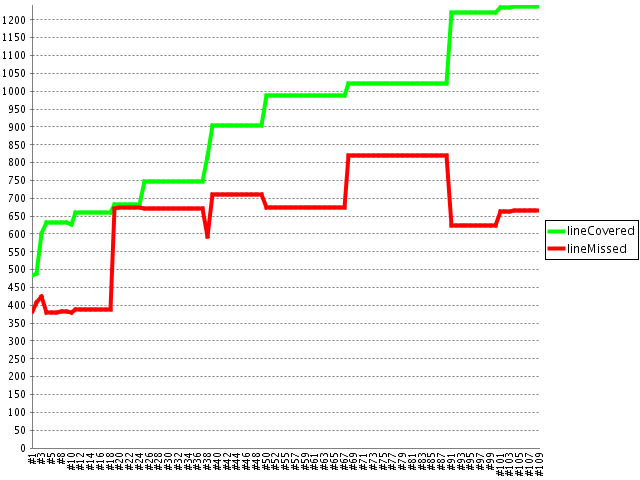
\includegraphics[width=\textwidth]{images/CodeCoverageTrendDev2}
    \caption{Code coverage trend for the development branch}
    \label{codecoveragetrenddev}
\end{figure}

We also underestimated the complexity of some features and thus did not wrote the tests for all cases with the first pull request of those features.
In that first basic implementation some of the cases were already implemented in part of the system but not actually called upon and made available from the front end.
We thus decided to first create a pull request for a basic version and thus split up the amount of changes.
Later, when the feature was further implemented, we added tests that would test these extra cases.

\subsection{Integration testing}
Everything a pull request was made, the changes were checked by a member of the team that wasn't the one requesting the merge.
This ensured that the changes made reflected the feature that was selected to be implemented.
The member of the team to check the code asked questions about some changes and checked if complex functions could be made more efficient.
Although we use checkstyle and findbugs to perform code analysis, they do not find everything.
So there is much value to achieve with a member of the team checking the code.

In figure~\ref{pullrequest-example} you can see an example of a pull request and how a team member commented on a part of the code.
The requesting team member responded on the issue and argued why he choose the implementation.

\begin{figure}[h]
    \centering
    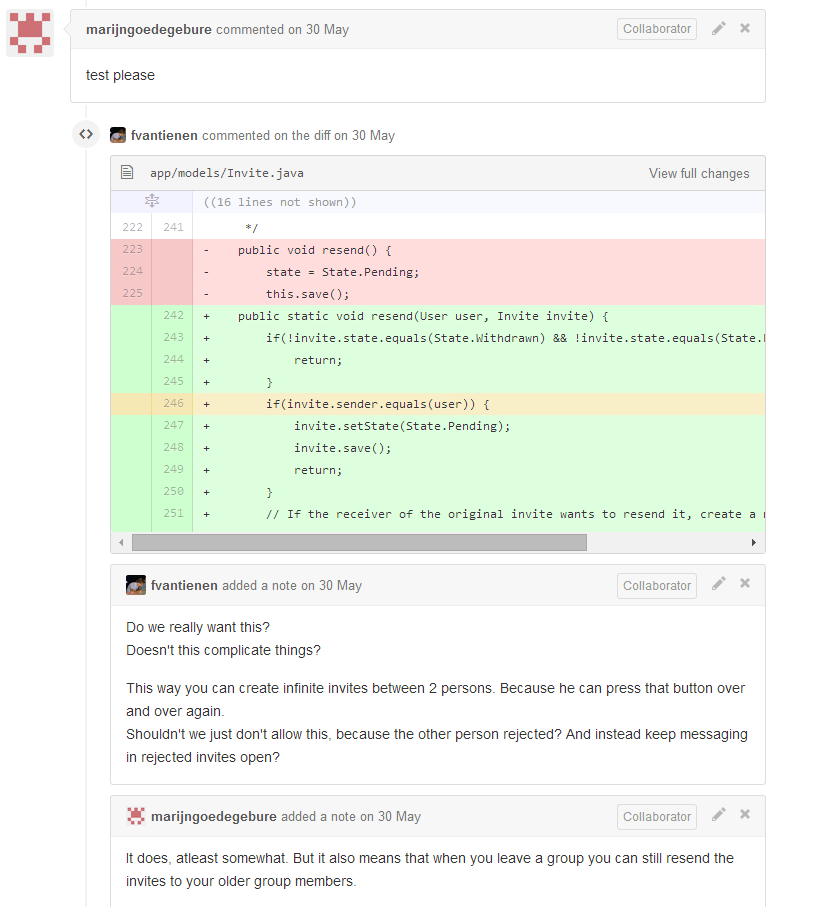
\includegraphics[width=\textwidth]{images/pullrequest-example1}
    \caption{An example of a pull request comment and reply.}
    \label{pullrequest-example}
\end{figure}

For an overview of the pull request and the comments that were made, you can find more information on the following website:
https://github.com/florisverburg/pm-impl/pulls

\section{Testing methods after the implementation phase}
The testing of the entire system is done after the implementation phase has been completed.
This is partly done by checking if the final product matches the requirements set.
It is also done by letting the target audience use the system and document the findings.
We will start with describing the user tests.

\subsection{User test}
The purpose of the user test is to test the system without the limiting factors of a development environment.
The system will be tested for his robustness in the different kinds of input a user can generate.
The test also let's the user make extensive use of the interface that we provided.
Any errors will be revealed by the user interaction.

To test the system we will be defining the people that are valid testing subjects and how we documented the various aspects of the test.

\subsubsection{The user}
We define a valid subject for our user test as a person that is part of the target audience (which we already defined in an earlier chapter).
The user should also be unfamiliar with the system.

\subsubsection{The test}
The user will be asked to test different functionalities which we will define beforehand.
We hand the user a document which lists the different actions that we want the user to do.
Before and after the test we let the user fill in a survey.
The survey at the start is about who the user is and the survey at the end is about what they thought of the system.
The surveys and instruction document can be found in the appendix.

\subsubsection{The user test results}

\subsection{Requirements test}
%Each of the requirements is listed and compared to the result

\section{Software Improvement Group Feedback}
\subsection{Intermediate feedback}
\subsection{Improvements}
\subsection{Final feedback}




\chapter{Conclusion}
\label{sec:conclusion}
During the past weeks we have created a platform where teachers can create the practicals associated with their MOOC and where students can enrol for practicals and form practical groups to work together on assignments.
This platform serves as a proof of concept for the various problems that were mentioned in the problem description.
One of the problems is the scale of MOOC's, which makes searching for a good group member is not a trivial problem.
To assist the student in forming a good group, the platform recommends possible group members to the searching student.

We split the project up in three phases: the orientation phase, the implementation phase and the final phase.
The project started off with the orientation phase in which the different aspects of the problem description were analysed.
During this time we looked into what kind of recommendation algorithm we will be using.
We also made an extensive list of requirements that helped us set out the different design decisions.
Lastly, we made a basic system design.
In the next phase, the implementation phase, we incrementally implemented the different features of the system.
At the end of the implementation phase we started the user tests.
With these user tests we tested the interface and basic usage of the system.
During the last phase we finished up the last features and we focused on documenting the project in this report.
We also received the feedback of SIG on the maintainability of our source code, one of the things done in the last phase was to improve the source code using this feedback.
The last thing to be done in the last phase is looking in what ways we can improve on the final product.
This is discussed in the future work section later this chapter.

%Uitleggen wat we in dit document hebben beschreven
This report documents the entire project.
We start with introducing the problem and our target audience.
Secondly, the report describes our supervisors, the different actors of the system, global goals, global requirements and detailed requirements.
Following this, we describe the project methodology we have chosen and we discuss how it panned out for us.
Per phase we describe the goal, planning and deliverables of the phase.
We also reflect on each phase separately.
In chapter 4 we describe the design we made of the system and how we implemented specific parts.
Things that we discuss in this chapter: Database diagram, class diagram, state diagrams, sequence diagrams, MVC, implementation of the recommendation algorithm and implementation of the invitation system.
Next, we describe the different kinds of testing that has been done during the project.
We start with describing the different kinds of testing that we have done during the implementation phase, followed by the testing that we have done after the implementation phase.
During the implementation phase we made use of unit testing and integration testing.
After the implementation phase we made use of a user test and requirements test.
Lastly, we describe the feedback that we have received from SIG and how we think to improve on this feedback.

\textbf{The final product, that will be presented, will be a working proof of concept which will fit closely with the specified target audience and demands of the assignment.}
To determine whether this goal has been met, we can look at the requirements.
The requirements have been set up with the target audience and the problem description in mind.
The problem description states the following important problems that need to be solved by the system:
\begin{itemize}
\item Difficulty finding a good practical partner.
\item Searching for a practical partner is a time consuming process.
\item Sub optimal solution, people often look for group members which share some interests.
While this often makes it easy to work together, this will not guarantee that you have a good functioning group with enough knowledge.
\end{itemize}

Looking at the requirements, we can definitely see that these problems are well represented by the requirements.
During the project we focussed on implementing these requirements.
It is no surprise that the resulting product is a proof of concept for the solutions that we have selected to solve the problems mentioned above.

To determine how well our proof of concept solves the problems we will have to look at to what extent we have implemented the requirements.
We will make that comparison in the other goals, since those goals were focussed  more on what the system should be able to do.

\textbf{We want to create a platform for searching other students and letting the students invite other students for a practical group.}

We have achieved this goal by creating a website and implementing an invitation system for this website.
Using this invitation system, students can search and invite one another.
This invitation system gives students the possibilities to invite both single students as groups of students.
It also gives groups the possibilities to invite both single students as groups of students.
The invitation system gives the user all the possible actions needed for the process of creating a practical group.

We can verify the completion of these features by looking at the requirements test.
The requirements clearly states which requirements have been implemented and which requirements have not.
The requirements test also clearly states that all the must and should haves concerning the creation of a platform for searching and inviting other students have been implemented.

\textbf{We want the final product to recommend good fitting possible group members to the students.
By "good fitting" we mean that there is some heuristic that we use to calculate whether two students would make a good practical group.
We want the final product to achieve more optimal solutions than the current situation}

In our research report we wrote extensively about what aspects are important to our recommendation algorithm.
Questions that we asked ourselves at the start of our research were:
\begin{itemize}
\item How does the algorithm determine a possible practical partner?
\item How does the algorithm make a difference between two possible partners and determine which one is a better fit?
\item How does the algorithm make use of the extra information provided if the could haves are implemented?
\item How does it make sure the partner that is recommended hasn't already been suggested?
\end{itemize}

We tried answering these questions using known techniques like knowledge-base recommendations, content-based recommendation, collaborative recommendation and demographic recommendation.
After doing research we concluded that the known techniques did solve all our problems.
We thus choose to select aspects of some techniques and combine these to a complete solution.
We decided upon the following aspects:
\begin{itemize}
\item The algorithm uses the idea of social interaction platform that is based off the platform that the Tinder app uses.
\item The algorithm uses a knowledge-based approach to deal with the various kinds of user information.
\item We use the geometric mean that is used by OKCupid's algorithm to calculate the differences and similarities between users.
\item We would like to make the algorithm robust for cold-start problems, the usage of a knowledge-based approach should help with this.
\end{itemize}

We do not have a guarantee of the performances of our algorithm, but we can say that our algorithm is perfectly tailored for the problems that were mentioned in the problem description.
We can improve on our understanding of the implemented algorithm and it's results by creating simulations.
These simulations would simulate the different actions of the system and will simulate both the use of the system as the use of the algorithm.
Due to the time limits of the project we did not get to implementing these simulations.

Using the requirements test of chapter 5 we can say that we have done a good job implementing the must and should haves that are focused on these problems.
The only thing we have fallen short in, is the fact that we deal with a wide target audience.
MOOC's are open to all people and we have not spend enough time writing an explanation of the system.

\textbf{We want the final product to have a high maintainability.
This means that we would like to achieve an above average score with the Software Improvement Group test.}
Maintainability is very important in creating a software product, because it is important to easily solve defects, replace worn-out components, meet new requirements, etc.
While programming, all these aspects are very important.
In chapter 5 we have discussed the SIG feedback.

To have an above average score, you need a score of out of five stars in the SIG test.
In our first submission we almost scored four stars.
The SIG does not just give you a score, it also gives you feedback on possible improvements.
Using this feedback we want to improve our system and try to score a four or even a five out of five stars.
This will be further discussed in our presentation.
For now we are happy with the three stars that we have scored.


%% Use letters for the chapter numbers of the appendices.
\appendix

%\input{appendix-a}
\chapter{Appendix A - Plan of Approach}
\section*{Preface}
This document is the Plan of Approach report that has been written for the Peer Matching assignment for the Bachelor Project course.
The assignment was issued by Dr. L.J.M. Rothkrantz of the TU Delft.
In this document, we will outline the Plan of Approach for this project.
In the firstsection* we will introduce the assignment and explain why it was issued.
In the second chapter we will describe the current situation, the goal of the project, the project assignment and the deliverables.
In the third chapter we will define our approach and planning for the time that is available to us.
In the fourthsection* we will define the project approach, who will be working on the project, who is in charge of what and administrative procedures.
We will also be describing how we finance the  resource that we require, how we will report the progress and what technical resources we will be using.
In the finalsection* we will describe our approach to assuring quality of the final product.
\section*{Introduction}
In thissection we will provide an introduction to the assignment.
We will start by giving a company outline followed by giving a background and motivation of the assignment.
This will answer the question: why has this assignment been issued? 
\subsection*{Company outline}
The assignment is issued by Dr. L.J.M. Rothkrantz who is part of the Interactive Intelligence group in the Intelligent Systems department.
This department is located in the EEMCS faculty at the TU Delft.
The research mission of the Computer Science department is as follows:
"The research mission of Computer Science within the Faculty of EEMCS is to contribute to the advancement of science, engineering, and design in the broad fields of autonomous distributed systems and information analysis and interaction."\cite{cstudelftnl}

\subsection*{Background and motivation of the assignment}
Each year many students go to an university to follow the predefined bachelor and/or master programs, but not everyone has the time and intent to follow an entire program.
There is a demand from all sorts of people to be able to follow a course while their main occupation isn't that of a student.
For example: a working parent could be very interested in such a course.
That is why universities introduced MOOCs.

The basic idea of MOOCs is that students remote in place and time follow the lectures, can participate in a practical assignment and can make an exam.
If they score sufficient, they are rewarded with a certificate that states their success in the course.

The concept of the MOOCs is a very new concept that still has many areas to improve upon.
One of these areas is the area of practical assignments.
Currently, for a Computer Science MOOC at the TU Delft, multiple practical assignments are required.
The participants are required to form groups to make these assignments.
After the announcement the participants either use mail, Facebook or  Twitter to contact other people in order to form the groups.

We would like to improve upon this concept and try to provide a more fitting approach.
\section*{Assignment description}
In thissection we will describe the definition of our Peer Matching assignment. 
We will describe which people are involved in the assignment, what the exact assignment is and what the difficulties can be.

\subsection*{Client}
The assignment was written by Dr. L.J.M. Rothkrantz of the TU Delft and is our main client.
Dr. L.J.M. Rothkrantz asked Dragos Datcu from the TU Delft to advise us on our design and implementation of the Peer Matching assignment.

The target users of the system are MOOC participants and MOOC teachers, specifically for the Computer Science courses. The system is easily extendable to provide more different MOOCs then Computer Science courses, but will not be supported by default.

\subsection*{Contact information}
\emph{Team}

Marijn Goedegebure
\emph{(marijngoedegebure@gmail.com)}

Floris Verburg
\emph{(floris.verburg@gmail.com)}

Freek van Tienen
\emph{(freek.v.tienen@gmail.com)}

\noindent\emph{Project supervisors}

Dr. L.J.M. Rothkrantz

Dragos Datcu

\subsection*{Problem description}
MOOCs around the world are growing in size and thus the practical assignments need to be easy to manage.
The growth also means that it is more difficult for each participant to find a possible practical partner due to the large amount of people.
It also becomes really difficult to find the correct partner or group members when you don't see each other during courses and haven't even met most of the people from your course.

Most of the time participants of MOOCs are searching group members on social media like Facebook or Twitter.
They just try to look through some of the participants names in the course, search for them on-line through social media and check if they are a capable partner or group member.
This approach takes a lot of time and most of the time there are too much MOOC participants to go trough all of them.

Next to the fact that this process is very time consuming, this process also often leads to a sub optimal solution.
This is due to the problem that people often look for partners of group members which share the same interests.
While this often makes it easy to work together, this will not guarantee that you have a good functioning group and enough knowledge inside the group.

We would like to improve upon this process by creating an application that can be used to create practical groups without the participants being required to go search intensively trough all the participants.
Participants should be able to easily access the application, fill in some relevant information about themselves and then be recommended possible practical partners or group members.

The interaction with the system has some difficulties.
If we want to get some information from third parties, we are required to use the information in a way this third party delivers the data.
There can be difficulties processing this data.
  
The recommendation of possible group members can be quite difficult too.
One of the problems we are facing is the question: What user information is useful to determine whether two people can be good practical partners?

\subsection*{Goal}
To provide an overview of what the software must be capable of, we define four global requirements for the system.
By defining these four global requirements we provide a foundation of what the system must be able to do.
\begin{itemize}
\item MOOC teachers must be able to create, manage and edit courses for which participants of their MOOC are able to register.

\item MOOC students must be able to register and deregister for a MOOC practical assignment.

\item The system must be capable to use personal data provided by the user to find a suggestion of an appropriate practical partner or group member.
It must be possible to adjust the definition (parameters) of the appropriate practical partner or group member, and search trough several suggestions.
\end{itemize}

\subsection*{Assignment formulation}
During the course of this project we will develop a Peer Matching system for finding appropriate practical partners or group members during MOOCs practical assignments.
To be able to find an appropriate practical partner or group member, we split up the assignment in two main areas of focus:

\textbf{The basic system} makes it possible to register to MOOC practicals, find and create practical partners or group members, and communicate with other participants.
The research in this area focusses on which information a participant would like to know when choosing a practical partner or group member.

\textbf{The algorithm} makes it easier for the users to search through all the available practical partners by giving suggestions of appropriate practical partners or group members.
Here the research is focussed on how to find suitable group members or practical partners, based on skills and personality.

\subsection*{Deliverables}
At the end of the project we will deliver a working prototype of the Peer Matching system, containing as much requirements as possible.
Because of the complexity of the Peer Matching algorithm and the short timeframe of 10 weeks, we choose to develop a prototype instead of a full working product.
We also choose to focus mainly on MOOCs from the study Computer Science, because the development team has more experience with these courses which makes it possible to make a more feasible Peer Matching algorithm.

\subsection*{Risks}
We have concluded the following main risks:

\begin{itemize}
\item Finding a suitable algorithm for matching practical partners and group members could be very difficult to evaluate and requires a lot of time.
This is because it is very difficult to define a "suitable" match between practical partners and group members based on skills and personality.
Every student is different and has its own preferences about a "suitable" practical partner or group member.
This makes it almost impossible to evaluate if the algorithm gives correct suggestions to the students.

\item Overestimating our knowledge and underestimating the time required for tasks.
Since this is a common problem with Software Engineering there is a good change that this will also be happing to us.
Estimating the knowledge in de software design team is very difficult because it relies on too many factors.
Because of that estimating the time required for several tasks is very hard.
\end{itemize}

\section*{Approach and time schedule}
In thissection we will be describing the methods, techniques and tools that we will be using to develop our application.
We will also be giving a global overview of the planning.

\subsection*{Methods and techniques}
We will be developing our application in the programming language Java.
We will combine this with the Play framework to provide us with a solid basis with which we can develop our web application.
Next to this we will be using scrum as our software development, more on that in the appropriatesection*.

\subsubsection*{Applications and technologies}
We will being using the following applications and technologies:
\begin{itemize}
\item IntelliJ IDEA, is our Integrated Development Environment (IDE) which will facilitate the development and testing of our code.
IntelliJ will be integrated with the Play framework which will be helpful during development.
\item GitHub, is our on-line code and documentation repository.
It provides for a version control system, an issue tracker and code review possibilities.
We will be using it to store all our code and documentation's code (LaTeX).
\item Cloudbees
Cloudbees will be used to run our test environment, our continuous integration and the release environment.
It uses Jenkins for the continuous integration.
\item Play framework
The play framework gives us the possibility to easily create a web application using Java.
\item Findbugs is a plug in for Cloudbees and IntelliJ that gives us the possibility to let our java code be checked for small bugs using static analysis.
\item JaCoCo is a plug in for Cloudbees and IntelliJ that provides us with data analysis about our code coverage.
\item Checkstyle is a plug in for Cloudbees and IntelliJ that checks the code for coding standards.
This makes it ideal to enforce the coding standard for our project.
\end{itemize}

\subsubsection*{Software development method}
We will be using scrum as our software development method.
Scrum is based on the agile software development framework which can be used to manage software projects.
We choose scrum because of its flexible approach to software development.
We do not have the time to research all of the aspects of the system.
Scrum gives us the possibility to react to changes of requirements, but also to react to new insights given by our increasing understanding of the system as time progresses.
We will define the different roles associated with scrum (e.g. the product owner, development team, scrum master) in the nextsection*.

\subsection*{Planning}
We have set up a global planning that splits up the project in phases.
Each of these phases has deliverables attached to them.
We will be mentioning our goals for each week.
Other important dates are also added to the planning.

\subsubsection*{Phase 1, Set up and research}
During the first phase we will be researching the requirements of the system and which requirements are essential for the application and what requirements are not.
We will also be looking into the set up of the project for our implementation phase.\\

\noindent{Week 1: 21-04-2014 - 25-04-2014}\\
Drafts of Plan of Approach and literature study, setup of the development environment.\\
\noindent\emph{Week 2: 28-04-2014 - 02-05-2014}\\
Finished Plan of Approach, literature study, first system design.

\subsubsection*{Phase 2, Implementation}
During the second phase we will be developing the application.
During this time we will be using Scrum to support our development.
During week 3 to 8 we will be developing the application.
During this time we won't have big deliverables, but we will be using the weekly meetings with our supervisors to measure our progress.\\

\noindent\emph{Week 3: 05-05-2014 - 09-05-2014}\\

\noindent\emph{Week 4: 12-05-2014 - 16-05-2014}\\

\noindent\emph{Week 5: 19-05-2014 - 23-05-2014}\\

\noindent\emph{Week 6: 26-05-2014 - 30-05-2014}\\
Start of the acceptance testing.

\noindent\emph{Week 7: 02-06-2014 - 06-06-2014}\\
End of the acceptance testing, first draft of the final report and send code to SIG for review.

\subsubsection*{Phase 3, Final report and presentation}

\noindent\emph{Week 8: 09-06-2014 - 13-06-2014}\\
Final development week, final draft of the final report.

\noindent\emph{Week 9: 16-06-2014 - 20-06-2014}\\
Send code for final review to SIG, send final report to supervisors for review, creation of the presentation.

\noindent\emph{Week 10: 23-06-2014 - 27-06-2014}\\
Presentation
\section*{Project approach}
In thissection* we will be explaining our approach to the project.
This begins with by defining the stakeholders of the project and what roles they will be having during the course of the project.
Following this, we will be explaining the administrative processes that will be used to monitor the project and to make sure that it will achieve the goals set.
Next, we will explain the means by which we finance the resources we use.
We will also define the ways in which we report our progress to the client.
Lastly, we will define the resources that we will be using during the project.

\subsection*{Stakeholders}
The following table lists the different group members, their roles and a short description.
This description describes the role and responsibilities of the group member.\\
\begin{tabular}{|l|l|p{5cm}|}
\hline
Name & Roles & Description\\
\hline
Freek van Tienen & Lead Development & Responsible for implementation phase.\\
\hline
Floris Verburg & Scrum master and Quality Assurance & Responsible for the Scrum process, the quality of the code and test coverage.\\
\hline
Marijn Goedegebure & Project Manager and Reports & Manages the project and ensures that the requirements are met.\\
\hline
Leon Rothkrantz & Client, Group Mentor and Supervisor & Supervises the project, aides the group with difficulties and has issued the assignment.\\
\hline
Dragos Datcu &  Group Mentor and Supervisor & Supervises the project and aides the group with difficulties.\\
\hline
\end{tabular}

\subsection*{Administrative processes and reporting}
In thissubsection* we will be describe the administrative processes that we will be using to make sure that the project will achieve the goals set.
\subsubsection*{Monday meetings}
We will have weekly meetings on Monday with just the group members to determine the weeks deliverables and talk through their requirements.
For each week we set up an agenda at the start of the meeting with all the things we would like to talk about.
During the meeting one of use will make minutes about the meeting which will be available to all the group members on the google drive.
During this meeting we will single out tasks that can be done and add those to a google drive file.
This google drive file is a log that has all of the tasks that have been done, are in progress and need to be done.
Each task has an assigned group member, a phase, a category, a yes/no if it is finished, a deadline and a finishing date.
When a task is finished the finishing date is filled in and the task is set to finished. The group member that just finished his task can now use the log to determine what to do next.
This log will also be used as the backlog for the scrum period.
\subsubsection*{Friday meetings}
We will have weekly meetings on Friday with our supervisors.
During this meeting we will be talking about the progress that has been made past week and what we plan to do next week.
We also talk about design decisions during these meetings.
There will also be minutes documenting the important information and decisions of this meeting.
\subsubsection*{Development period}
During the development period we will be having daily meetings, as prescribed by Scrum.
These short meetings will follow the Scrum paradigm.

\subsection*{Financing}
We do not have a budget provided so our project must use open source software and free to use services.
All of the tools and techniques that we use follow this rule.

\subsection*{Reporting to the client}
We will use the Friday meetings to report our progress to the client (and supervisors).
The deliverables that we set will be sent to the supervisors for review.

\subsection*{Resources}
We will be using the different meeting rooms and public studying areas as our working environment.
Although not perfect, it will be enough for the short duration of the project.
The meeting rooms provide for a good place to hold meetings and work together as a group.
The public studying areas are a good place to work alone on a task.

\section*{Quality assurance}
For quality assurance we use several tools and techniques, to make sure our code is maintainable and is well documented.
In thissection* we will first describe some of the techniques we will use and explain why they are useful for quality assurance.
Next we will describe how several tools are providing use useful help and knowledge about our quality.

\subsection*{Techniques}
As described before we will use scrum as our software development method, which will give us the opportunity to write tests very early in the process.
Due to the fast scrum cycles of one week and splitting the software in small features, we can test each feature in the same scrum cycle.
This way we will detect bugs and programming faults very early.
We will also detect possible problems in the group process early.

Next to scrum we will make use of Git branches to separate our feature implementations in different branches.
When a feature is completely tested and reviewed by another member of the programming team, it will be merged into the staging branch.
For this, we will use pull requests on Git, so everyone of us must review the changes before they will be added to the staging branch.
After that acceptance testing will be done on the staging branch and when all tests are passed it will be merged into the master branch.
This will always assure that we have a stable release available in the master branch.

As last technique we will use unit testing together with acceptance testing with our client and future users of the system and together with user testing.
Unit testing will be happing during each scrum cycle, and will be required for each feature to be merged into the staging branch.
Acceptance testing will happen in the last two weeks of our project implementation and will give us feedback on which requirements we finished or didn't finish.
User testing also will happen in the last two weeks of our project implementation.
These tests will give us feedback on the accessibility of our system and if the system interacts in a natural way.

\subsection*{Tools}
For quality assurance our main tool will be the Jenkins (Cloudbees) continuous integration testing environment.
This environment gives us the opportunity to automatically perform several testing techniques and code analysis during each push to the Github repository.
In this environment we will run several tools we will explain in the following paragraphs in more detail.

At first all our Unit test will be run on Jenkins, which will give us fast feedback about the functionality of classes and functions.
Bugs can easily be found, and when code is changed later on each test will be run again to make sure it keeps on working.

Next we will run Findbugs to statically analyse our code for small bugs, and wrong naming conventions.
This will not make sure there are less bugs in our code, but at least will give a helping hand in finding bugs very easily.

After Findbugs we will run JaCoCo, which will give a really good insight in the data analysis of our code coverage.
It will help use find parts of code where more testing needs to be done.

As last we will run Codestyle, to make sure that every programming holds itself to the same conventions.
Codestyle will rive a report of the errors in the conventions and need to be checked before pushing to staging,
This will make sure our code is more maintainable, because it provides more easy to read and understand code.

\chapter{Appendix B - Assignment}
This was the first version of the assignment. After the start of the project, the assignment has changed.

\section*{Project description}

It is well known that many students come to the University to visit lectures because it provides the opportunity to meet peers and to have discussions also about less academic topics. The meeting place at the University is partly replaced by a virtual meeting place. Students report about their daily activities, opinions, problems using social media. At this moment social media play a limited role in the academic process of teaching and learning. But social media offer great opportunities, especially around the development of MOOCS (Massive Open Online Courses).The basic idea of MOOCS is that students remote in place and time follow the lectures, they can use social media as academic communication media, where students discuss about their study activities, put forward their questions and get help and support from peers. The question is how to find the best matching peers especially peers outside TUDelft. Inspecting all the profiles via Facebook is too time consuming. Supporting matching tools are needed. At this moment there many sites finding the best matching partner, our interest is finding the best matching study partners. A possible option is to extract features from student profiles via FaceBook , take care of preferences and expert knowledge and train classifiers or other matching technologies. Students involved in the peer matching project are supposed to communicate via social media. But at the end of the project there will be a written report. The TUDelft supervisor Leon Rothkrantz is involved in supervising students for many years. Currently he participates in an European project FETCH aimed at the development of new didactical models for distant learning. This gives the current Peer matching project an European dimension and offers cooperation with students from other European Universities.

\section*{Company description}

The TUDelft is well known, so no additional info is provided. At this moment there is a lot of interest in the development of MOOCS. The Board of the University (Anka Mulder) supports the developments for many reasons. In the framework of The European Life Long Learning Program TUDelft is a partner in the FETCH project (Future Education and Training in Computing). More than 55 European Universities are involved in this project. There is a special Work Package on the use of social media in distant learning. Prof. drs. dr. L.J.M. Rothkrantz is the coordinator of this project. There are possibilities for students to take part in this project and present their work on Educational Conferences organised by the project.

\section*{Auxiliary information}

The company FeedbackFruits will be represented by Ewoud de Kok (ewoud@feedbackfruits.com +31630496917). The company is cofounded by TUDelft graduates (computer science). The have experience in developing software products according to well known standards. last years many students did an internship at the company He will have the role of case holder or client of the project. An interesting aspect is to study how online educational platforms will change the content and didactical aspects. It is now a fact that many students are online almost the whole day. Regular courses at the University are too static, boring and most important not interactive. It proves that even workgroups and interaction during classes are less effective. It is difficult to measure the effectivity/efficiency and to make effective changes in the way of teaching.Online courses have a broad spectrum of didactical forms. It ranges from video lectures, courses with quizzes and tutorials at regular times, courses modelled as games, and a lot of gimmicks which gives learning a lot of funs Online courses have a lot of social activities (not only knowledge transfer), students will be stimulated and enabled to help each other during hangouts and group meetings via Skype-like interfaces. This enables students to give feedback and discussions about the content, with or without the lecturer. The educational challenge is to integrate for example the use of social media in online courses. This will have a huge impact on the way Universities will offer educational and training material.
\\\\
Company: TUDelft, Fetch\\
TU Delft coach: Leon Rothkrantz\\
TU Delft coach email address: L.J.M.Rothkrantz@tudelft.nl\\
Company contact: Leon Rothkrantz\\
Company contact email: l.j.m.rothkrantz@tudelft.nl

\chapter{Appendix C - Research Report}
\section*{Preface}
This document is the research report that has been written for the Peer Matching assignment for the Bachelor Project course.
This course is the last project based course of the Bachelor of Science at the TU Delft in the Netherlands. The assignment was issued by Prof. drs. dr. L.J.M. Rothkrantz of the TU Delft.
The report provides a summary of the requirements that are set for the system and will provide for a literature study about different possible algorithms to solve the peer matching problem presented in the problem definition.

\section*{Introduction}
Many students go to an university each year to follow the predefined bachelor and/or master programs, but not everyone has the time and intent to follow an entire program.
There is a demand from all sorts of people to be able to follow a course while their main occupation isn't that of a student.
For example: a working parent could be very interested in such a course.
That is why universities introduced MOOCs.

The basic idea of MOOCs is that students remote in place and time follow the lectures, can participate in a practical assignment and can make an exam.
If they score sufficient, they are rewarded with a certificate that states their success in the course.

The concept of the MOOCs is a very new concept that still has many areas to improve upon.
One of these areas is the area of practical assignments.
Currently, for a Computer Science MOOC at the TU Delft, multiple practical assignments are required.
The participants are required to form groups to make these assignments.
After the announcement the participants either use mail, Facebook or  Twitter to contact other people in order to form the groups.

TUDelft has been a forerunner in the field of Open \& Online Education since 2007 and is one of the sustaining members of the OpenCourseWare Consortium and since 2013 charter member of the edX Consortium. 
In March 2014, the board of the TU Delft approved an innovation program to accelerate the development of open \& online education. 
The goal is to create a Delft Extension School that will bundle all open \& online courses for a global population of life long learners.

We would like to improve upon this concept and try to provide a more fitting approach.

\subsection*{Problem definition}
In this subsection* we will continue on the case provided by the introduction.
We will pinpoint the points we would like to improve upon.

MOOCs around the world are growing in size and thus the practical assignments need to be easy to manage.
The growth also means that it is more difficult for each participant to find a possible practical partner due to the large amount of people.
It also becomes really difficult to find the correct partner or group members when you don't see each other during courses and haven't even met most of the people from your course.

Most of the time participants of MOOCs are searching group members on social media like Facebook or Twitter.
They just try to look through some of the participants names in the course, search for them on-line through social media and check if they are a capable partner or group member.
This approach takes a lot of time and most of the time there are too much MOOC participants to go trough all of them.

Next to the fact that this process is very time consuming for every participant, it also leads to a sub optimal solution.
This sub optimal solution will be focussed on a group or set of partners which share the same interest and this doesn't say anything if they would form a good group.

We would like to improve upon this process by creating an application that can be used to create practical groups without the participants being required to go search intensively.
Participants should be able to easily access the application, fill in some relevant information about themselves and then be recommended possible group members.
Our peer matching tool is an add on for the MOOCs. 
It can be parallel used for every MOOC with group assignments.
The teacher can create a course in our tool to represent a MOOC.

The interaction with the system is a pretty straight forward application, but the recommendation of possible group members is more difficult.
One of the questions we are trying to answer is: What user information is useful to determine whether two people can be good practical partners?
We will also need to figure out a good way to recommend a practical partner, but still give the possibility to reject such a request.\\

\emph{We have two problems. First, how can we find appropriate matches for people? And second, how can we create optimal groups?}\\

These questions and difficulties will be answered in this report.

\section*{Introduction to requirements}
The following section*s will describe what requirements are set for the product.
This section* will define four global requirements who cover the entire project.
These requirements are then split up in the next two section*s, the first being the requirements for the basic system and the second being the requirements for the peer matching algorithm.
We choose to split these requirements up, because of the literature study required to further specify the requirements.
In these section*s, the global requirements are split up in smaller requirements.
It is easier to verify these smaller requirements for their completion and these requirements are more transformable to functions of the system.
We also assigned these requirements into their appropriate MoSCoW \cite{highsmith2001agile} method category.

\subsection*{Actors of the system}
In this subsection* we will clarify the different actors used in the system and throughout this report.
\subsubsection*{MOOC participant}
Due to the nature of the MOOCs, there are no requirements set for the participants.
Every person with an interest in the given course can enlist for the MOOC and should thus be able to register with our system.
\subsubsection*{MOOC teacher/MOOC administrator} 
The MOOC is organised by a professor of an university.
This professor will need to register with the system and create a MOOC.
\subsubsection*{Groups of participants}
This actor consist of two or more MOOC participants who accepted each other to their group.
These groups can be of variable size, set by the MOOC organiser.

\subsection*{Global Requirements}
To provide an overview of what the software must be capable of, we define four global requirements for the system.
By defining these four global requirements we provide a foundation of what the system must be able to do.
\begin{itemize}
\item  MOOC teachers must be able to create, manage and edit courses.
Participants of their MOOC are able to register to this course.

\item MOOC students must be able to register and deregister for a course.

\item The system must be capable to use personal data provided by the user to find a suggestion of an appropriate practical partner or group member.
It must be possible to adjust the definition (parameters) of the appropriate practical partner or group member, and search trough several suggestions.
\end{itemize}

\section*{Requirements}
This section* will mention the different requirements that involve the basic system which the actors interact with.
The section* starts with mentioning the possible types of user information the application can use and what requirements are associated with that.
Followed up by what actions are possible within the system.
After that the kind of system is limited by the requirements listed.
Lastly we will list the requirements set for the algorithm.
Each section* will use the MoSCoW model to divide the requirements in their appropriate categories.


\subsection*{User information}
\reqr{Must have}
\begin{itemize}
\item Users must have a viewable profile that can be filled with personal information.
\item Users must be able to enter the following registration information during registration: Full name, Email address, Password and Language.
\item Users must fill in their academic performances. Which knowledge, skills and completed courses does the user have?
\end{itemize}

\reqr{Should have}
\begin{itemize}
\item Users should be able to enter the basic user information, like: country, age, short description, skills, education, a picture and personality traits.
\end{itemize}

\reqr{Could have}
\begin{itemize}
\item Users could be able to use a personality test to determine their personality traits.
\item Users could be able to fill in their personality traits.
\item Users could be able to enter the following extended user information: preferred group role, role of the other group members, etcetera.
\item Users could be able to enter a predefined questionnaires.
\end{itemize}

\reqr{Would have}
%\begin{itemize}
%\item
%\end{itemize}

\subsection*{Usage of the system}

\subsubsection*{Actor 1: MOOC participant}

\reqr{Must have}
\begin{itemize}
\item The a potential participant (anyone who visits the site) must be able to view the different MOOCs without registering or logging in.
\item The participant must be able to inform him/herself about the usage of the application without registering or logging in.
\item The participant must be able to register to the application.
\item The participant must be able to log in to the application.
\item The participant must be able to register to the MOOCs which they were enlisted for (known to the administrator).
\item The participant must be able to view a possible practical partner.
\item The participant must be able to communicate with the possible practical partner to verify the matching.
\item The participant must be able to accept or decline the practical partner into his practical group.
\item The participant must be able to communicate within the group.
\end{itemize}

\reqr{Should have}
\begin{itemize}
\item The participant should be able to ask a currently existing group if he can join them.
\item The participant should be able to use their Linkedin profile to log in to the application.
\item In case the participant already has an account, the participant should be able to add the course to his profile using the teachers url.
\item The participant should be able to receive an invitation from a group.
\item The participant should be able to accept the invitation from a group.
\end{itemize}

\reqr{Could have}
\begin{itemize}
\item The participant could be able to set his preferences for his possible partner.
\item The participant could be able to search for other participants using information that is available in the profile.
\end{itemize}

\reqr{Would have}
%\begin{itemize}
%\item
%\end{itemize}


\subsubsection*{Actor 2: MOOC teacher/MOOC administrator}
\reqr{Must have}
\begin{itemize}
\item The administrator must be able to create a course and add this to his account.
\item The administrator must be able to open and close the participant registration for a course.
\item The administrator must be able to manage the list of participants and groups of participants.
\item The administrator must be able to create an url that he can use to invite the participants.
\end{itemize}

\reqr{Should have}
\begin{itemize}
\item The administrator should be able to set a deadline for a practical.
\item The administrator should be able to communicate with every participant.
\item The administrator should be able to communicate with the groups.
\end{itemize}

\reqr{Could have}
\begin{itemize}
\item The administrator should be able to grade the group for its practical.
\item The administrator could be able to provide for his own criteria for each of his course.
\item The administrator could be able to add different assignments to the application.
\item The administrator could be able to view what groups have finished what assignments.
\item The administrator could be able to grade the different assignments.
\item The administrator could be able to provide feedback for the different assignments.
\end{itemize}

\reqr{Would have}
%\begin{itemize}
%\item
%\end{itemize}


\subsubsection*{Actor 3: Groups of participants}
This actor consist of two or more course participants who accepted each other to their group.

\reqr{Must have}
\begin{itemize}
\item The groups must be able to communicate with each other using the application.
\end{itemize}

\reqr{Should have}
\begin{itemize}
\item A group should be able to view a possible group member.
\item A group should be able to invite a possible group member to join their group.
\item A group should be able to accept an request from a participant to join their group.
\end{itemize}

\reqr{Could have}
\begin{itemize}
\item The group could be able to select their preferences for the new group member.
\item The participants could be able to share files to other group members using this application.
\end{itemize}

\reqr{Would have}
\begin{itemize}
\item The participants would be able upload their source code to the application for verification.
\end{itemize}

\subsection*{Kind of system}

\reqr{Must have}
\begin{itemize}
\item The application must be easily accessible to both participants and course organizers.
\item The system must provide account management functionality.
\item The system must use a database to store the different data put in by the user.
\end{itemize}

\reqr{Should have}
%\begin{itemize}
%\item
%\end{itemize}

\reqr{Could have}
\begin{itemize}
\item The system could be able to be combined with practical systems already used by MOOC organizers.
\end{itemize}

\reqr{Would have}
%\begin{itemize}
%\item
%\end{itemize}

\subsection*{Peer matching}
\reqr{Must have}
\begin{itemize}
\item The algorithm must be able to use a list of users as input.
\item The algorithm must deal with continuous variation in amount of users.
\item The algorithm must be able to return one or more suggestions of practical partners to the user given a list of rejected users.
\item The algorithm must be able to return one or more suggestions of possible groups the participant could join.
\end{itemize}

\reqr{Should have}
\begin{itemize}
\item The algorithm uses basic user provided data (e.g. education, preferences) to build up a profile for a course participant.
\item The algorithm can calculate whether two people will be good practical partners using the basic user provided data.
\item The algorithm can return a possible practical partners using the basic user provided data.
\end{itemize}

\reqr{Could have}
\begin{itemize}
\item The algorithm uses advanced user provided data (e.g. asked questions, programming tests) to build up an extended profile for a course participant.
\item The algorithm can calculate whether two people will be good practical partners using the advanced user provided data.
\item The algorithm can return a possible practical partner using the basic user provided data.
\item The algorithm could be able to respond to the preferences of groups.
\item The algorithm could be able to respond to the preferences of a participant.
\end{itemize}

\reqr{Would have}
\begin{itemize}
\item The algorithm would have to be able to use information gathered from rejections to improve the matching.
\end{itemize}

\section*{Design choices}
In this section* we will be describing our choices for the design.
For each choice we will be arguing why we have chosen for this.
We will argue using scientific literature or the requirements.
We will first describe the choices we have made concerning the kind of system.
Secondly we will describe the choices we have made concerning the framework that we will be using.
Following this, we will be describing the choices we have made concerning the algorithm.

\subsection*{Global system design}
In the global system design we will be describing a first concept of the system.
In this concept we will describe the different actions, that different actors will need to be able to perform.

The first thing that has to be done is for the teacher to create an assignment in the application.
It must be possible for the teacher to open and close this assignment. 
While creating, the teacher has to define some properties of the assignment.
When the assignment is created successfully, a link is generated that can be sent to the students.

When the students open the link, they have a choice between logging in or registering.
For logging in and registering, the student could use LinkedIn, so a lot of data is gathered automatically.
We can also look for LinkedIn alternatives, like Yammer and Ututi, which are non-commercial.
After filling in the basic information, the student must provide information about his personality.
This can be done by means of an questionnaire.

After logging in, the assignment can be added to the profile of the student.
After adding the assignment to the profile, some recommendations are provided.
The student can form groups by means of this recommendations.

\subsection*{Web application}
Our main decision about choosing to make a Web application was relatively simple.
This is due to the fact that MOOCs itself are also Web applications, which are available for everyone.
Because our application is specifically designed for MOOCs it should also be widely available for all the MOOC participants.
One of the best ways to do this is by developing a web application.

\subsection*{Framework}
Because Web applications are getting more and more popular, a lot of frameworks are appearing which we could use for our Peer Matching system.
Choosing the right framework is therefor really difficult, because they are hard to compare and not a good way to say which is better.
We therefor listed a couple of frameworks which we had experience with, to make sure we have a lot of knowledge available in our programming team.

We first started looking at the PHP based Kohana Framework\cite{kohana}.

The Java based Spring Framework\cite{spring} was also a possible solution.
Spring Web Flow builds on Spring MVC and allows implementing the "flows" of a web application.
The programming team doesn't have that much experience with the Spring Framework, but because they are all well known with the Java programming language it shouldn't be a problem.
It has a lot of useful features like an ORM (Object-relational mapping), transaction management and a MVC setup.
This makes the Spring Framework a good choice.

Next we started looking at the Python based Django Framework\cite{django}.
Django is a high-level Python Web framework that encourages rapid development and clean, pragmatic design.
But because the programming team didn't have that much experience with both Python and Django, we chose to avoid learning a totally new programming language and framework.

The last framework we looked at was the Play Framework\cite{play}, based on the programming language Java and Scala.
Play is a high-productivity Java and Scala web application framework that integrates the components and APIs you need for modern web application development.
The Play Framework looks a lot like the Spring Framework, it includes the same features and is also MVC based.

To conclude, we chose the Play Framework to work with. All of the team members already had experience with programming in Java. One of the team members also had worked with the Play Framework before, so we had some experience with this framework in our group.

\subsection*{Literature survey recommender systems}
Using the requirements stated in the previous section* we see that the requirements all state the need for the handling of a specific set of input and outputting the needed information.
The requirements do not state any limitations about the inner workings of the algorithm.
Some questions remain:
\begin{itemize}
\item How does the algorithm determine a possible practical partner?
\item How does the algorithm make a difference between two possible partners and determine which one is a better fit?
\item How does the algorithm make use the extra information provided if the could haves are achieved?
\item How does it make sure the partner that is recommended hasn't already been suggested?
\end{itemize}
Due to the unique requirements set to how the system works, we need to look for all kinds of different algorithms that could help us solve our problem.
Because of the unique requirements, these techniques will probably not solve the entire problem, but we can possibly use parts of these algorithms to formulate our own solution.

We have done a literature survey into recommender systems since these kind of systems are closely related to what we want to achieve.

As can be read in these papers \citep{Breese1998},\citep{Peter2007}, there are roughly five kinds of algorithmic recommendation approaches:

\begin{itemize}
\item Demographic filtering \citep{Peter2007}
\item Collaborative filtering \citep{Peter2007}\citep{Breese1998}
\item Content-based filtering \citep{Peter2007}
\item Knowledge-based filtering \citep{Peter2007}\cite{burke2000knowledge}
\item Hybrid filtering \citep{Peter2007}
\end{itemize}

The following image supports the existence of these five classes.
The image shows how the different classes use different kinds of resources.
Next to these recommendations we added a subsection* for the mentioning of other possibilities that we encountered while researching the subject.
We will now first discuss each of the techniques and what aspects are usable and what aspects are not.
\makebox[\textwidth]{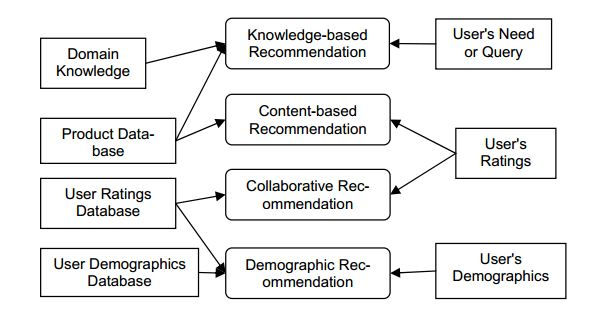
\includegraphics[width=12cm]{Images/RecommendationDomain}}

\subsubsection*{Demographic filtering}
In the paper Privacy-preserving demographic filtering\cite{aimeur2006privacy} demographic filtering is explained.
Recommender systems based on demographic filtering aim at categorising users based on their demographic information and recommend services accordingly. 
More precisely, demographic information is used to identify the types of users that like similar services. 

Demographic filtering can be used by any recommender system that offers services by using data on individual users. 
The key element of demographic filtering is that it creates categories of users having similar demographic characteristics, and tracks the aggregate behaviour or preferences of users within these categories. 
Recommendations for a new user are issued by first finding to which category he belongs and then by applying the aggregate preferences of previous users in that category.

In the paper A framework for collaborative, content-based and demographic filtering\cite{pazzani1999framework} an example is provide. 
For example, Table \ref{table:dfexample}  shows information on the age, gender, education, etc. of people that rated
a restaurant together with their rating of the restaurant. 
One might expect to learn the type of person that likes a certain restaurant. \\ 

\begin{table}[h]
    \begin{tabular}{|l|l|l|l|l|l||l|}
    \hline
    ~     & gender & age & area code & education & employed & Dolce \\ \hline
    Karen & F      & 15  & 714       & HS        & F        & +     \\ \hline
    Lynn  & F      & 17  & 714       & HS        & F        & -     \\ \hline
    Chris & M      & 35  & 714       & C         & T        & +     \\ \hline
    Mike  & F      & 40  & 714       & C         & T        & -     \\ \hline
    Jill  & F      & 10  & 714       & E         & F        & ?     \\ \hline
    \end{tabular}
\caption{Demographic filtering example}
\label{table:dfexample}
\end{table}

\noindent We could use data like these to recommend similar groups for people with the same demographic background.

\subsubsection*{Collaborative filtering}
The book Adaptive Web \citep{Peter2007} describes what collaborative filtering techniques are.
He says that these techniques generally involve matching the ratings of a current user for objects with those of similar users.
In this way it produces recommendations for objects that the users has not yet rated or have not been seen by the active user.
Traditionally, the primary technique used to implement a collaborative filtering is the use of k-Nearest-Neighbor (kNN) algorithm.
This algorithm compares a target user's profile with the historical profiles of other users in order to find the top k users who have similar tastes or interests.

Examples of collaborative filtering algorithms are found in the on-line dating branch.
An example that provides some insightful information about the subject is OKCupid.
The video ,that can be found on the website\cite{okcupid}, describes the workings of the OKCupid algorithm.
The OKCupid algorithm uses the geometric mean.
This is a type of mean or average, which indicates the central tendency or typical value of a set of numbers.
OKCupid's algorithm is an algorithm that uses questions and preferences to determine whether two people would make a good pair.
Instead of the questions they ask, we could fill in our own questions or values.
The geometric mean would still give an overall score for the combining of two people.

\subsubsection*{Content-based filtering}
The book Adaptive Web \citep{Peter2007} also describes what content-based filtering techniques are.
He describes content-based filtering systems as systems where in a user profile represents the content description of items in which that user has previously expressed interest.
The content description of items are represented by a set of features or attributes that characterize that item.
The recommendation in these kind of systems usually consist of comparing unseen or unrated items with the user profile.
Items that overlap with the interests of the user are recommended.

The paper Using Content-Based Filtering for Recommendation \cite{van2000using} describes an example of a recommender system that uses user information to determine what to recommend.\\
In this paper it becomes clear that a built up user profile can give a much better recommendation than a starting profile.
Although this can work for many applications, this means that the user needs to build up a training set.
The first couple of recommendations could be possibly bad and this is not in the users interest.
The user wants the best recommendation from the start.
Although it might look like content-based filtering can not be used for our domain, we would like to keep them in our thought as a possible way to improve upon the algorithm.
By using the user's history we can improve the recommendations by listening more to the users preferences.

\subsubsection*{Knowledge-based filtering}
In the book Adaptive Web, they also mentioned knowledge-based filtering as a class of recommendation techniques.
This is supported by a paper called Knowledge-based recommender systems \cite{burke2000knowledge}.
In this paper they describe it as a recommender system that uses knowledge about users and products to generate a recommendation.
It will use this knowledge to have a different approach to the generation of a recommendation and the user.
Knowledge-based recommendation systems do not have the problem of a so called cold-start problem.
The cold-start problem is the problem when a learning-based system does not have enough information to provide for a proper recommendation.
Learning-based systems are systems that learn from each user or product added to the system.
With each step they learn more about the users that are in the system and their preferences.
This can occur when a new user is registered to the system, a new product or when there are only a few current users.
This is a big advantage and is something we should keep in mind when designing our algorithm

One of the downsides of knowledge-based filtering is that it can't learn.
It will always be limited to the knowledge it has.
An expert can improve the knowledge the system has, but it will not do so autonomous like a learning-based system.

\subsubsection*{Hybrid filtering}
Adaptive web sites offer recommendations to the user by using a well studied technique.
This technique can either use collaborative, knowledge-based and content-based recommendation, but it can also use a combination of these techniques.
These kind of systems are called hybrid filtering techniques.
Each of these techniques has its own strength and weaknesses and by combining these researchers try to improve the performance of the techniques.
The resulting systems are called hybrid recommender systems and are defined as the combination of two or more of the different recommendation techniques.

A variety of techniques have been proposed as the basis for hybrid recommender systems: collaborative, content-based, knowledge-based and demographic techniques.

The learning-based techniques (collaborative, content-based and demographic) suffer from the cold-start problem.
Most hybrid recommender systems are combining techniques to deal with the cold-start problem.
This is something we need to keep in mind when designing our algorithm.

The converse of this problem is the stability versus plasticity problem.
Once a user's profile has been established in the system, it is difficult to change one's preferences.
Many adaptive systems make the older ratings have less influence and thus prevent the unresponsiveness of the system.

We can use a combination of different techniques, and thus have a hybrid filtering, to have a resulting algorithm that perfectly adheres to the requirements.

\subsubsection*{Other possibilities}
Recommender system all try to use data that has been collected to improve their recommendations, but there are other approaches to the matching problem.
A great example of an user based approach is the Tinder mobile-app.
This application allows users to get in contact with other people.
They only provide for a platform where the user can view people who are near you and adhere to some basic requirements (E.g. age limit and amount of kilometres away).
The user is shown a small profile of a potential match and let the user decide whether it is a go or not based on that info.

We would like our user to decide upon skills that are not very applicable to the Tinder format.
Another downside of the format is that it does not provide for a way to influence the outcomes of the groups.
For example, the administrator should be able to set values for the different skills that are advised for each group.
Lastly, we would like to narrow down the possible people an user will see to the ones that could be a positive addition to his group.
Although we can not use the entire format, we can use the accepting and/or rejecting of a possible group member.
It is also a good idea to let the possible group members talk to each other before they have to decide to join one's group.

\subsubsection*{Conclusion}
Each of these techniques are very interesting for having a good recommendation algorithm, but we do not have the time with this project to expand so vastly on the subject.
We will thus have to simplify the problem to something where for we can implement a basic recommendation algorithm and that still adheres to the requirements.\\
We concluded that the techniques weren't appropriate for the requirements that were set.
There are three reasons why the techniques mentioned above aren't appropriate for our solution.
First is the fact that the requirements state the need for the administrator to be able to influence the group characteristics.
Secondly the requirements state the possibility that the participants could be able to influence the recommendation.
Lastly not every method is able to easily provide for groups of different sizes.
The techniques mentioned above do not provide for the flexibility that we require.
We are best suited with an algorithm that can easily be implemented with a basic result and can easily be extended with extra functions.

\subsection*{The Algorithm}
Following up on the literature survey we need to decide what aspects of what techniques can be used to construct an algorithm and to determine how it will be used.
That is why we took another look at the requirements and how the different actors should interact with each other.
During this evaluation we thought up a algorithm that combines multiple known techniques that adheres to the requirements.

\subsubsection*{Aspects}
We decided upon the following aspects:
\begin{itemize}
\item The algorithm uses the idea of the social interaction platform that is based off platform that the Tinder app uses.
This part of the Tinder app provides for all the interaction possibilities needed for our system.
We only need to extend upon the creation of groups.
\item The algorithm will use a knowledge-based approach to deal with the various kinds of user information.
It is important to use the proper scales for each information type, else the algorithm can not properly determine whether two people would be good group members.
\item We use the geometric mean that is used by OKCupid's algorithm to calculate the differences and similarities between users.
By using this we can accurately determine how much two people defer from each other.
Using this data, we can determine who would and who wouldn't be good group members.
\item We would like to make the algorithm robust for the cold-start problem, the usage of a knowledge-based approach should help with this.
\end{itemize}

\subsubsection*{What does the algorithm do?}
The algorithm will be used to recommend a possible group member to a person.
It will do so by analysing information the user has filled in.
This information will be compared to other users to determine their similarities and differences.
The algorithm will then calculate how good of a group member others users are.
While computing this it will track the top partners to eventually return these to the user.
It will do so by combining the two group members and compute a resulting value for each information property.
Whether two user form a good group can then be determined by comparing the resulting values with predefined values.
These predefined numbers can either be set by the administrator or later adjusted by the searching participant.

\emph{Formal description of the algorithm}
There are two cases in which the algorithm should be able to recommend a new group member:\\
\emph{A single participant searches for a first group member}
Given m properties and n participants currently enlisted to the course the algorithm will search for a possible practical partner for participant X.
The algorithm determines for each possible practical partner how the creation of a group of that pair would bring them closer to the predefined numbers.
It will do this by taking the average for each property and taking the difference between this average and the predefined number.
It will then sum these differences and take the m root of this number.
This will result in an number that represents the overall difference between the group of the two participants and the predefined numbers.
A group with a low overall difference means that the two participants form a group that as closely meet the predefined numbers as possible.
During this calculation the algorithm keeps track of the top possible practical partners which it will return as a result to the participant.

\emph{A group searches for a new group member}
The second case is similar to the first, the calculation is completely the same.
The only difference is that you do not start with a participant X, but with a group of participants.
The properties of these participants are already averaged per property.
This results in a number per property which can be used by the algorithm mentioned above.

\subsubsection*{Possible improvements of the algorithm}
\begin{itemize}
\item The user can use extra properties (which the administrator can't define) to further specify their groups.
\item The user can adjust the predefined numbers (the predefined numbers of the administrator are not required).
\item The algorithm uses the group size to ensure that there are more versatile people in a group.
\item The algorithm can incorporate a content and/or collaborative-based recommendation.
\end{itemize}

\chapter{Appendix D - User test Google form}
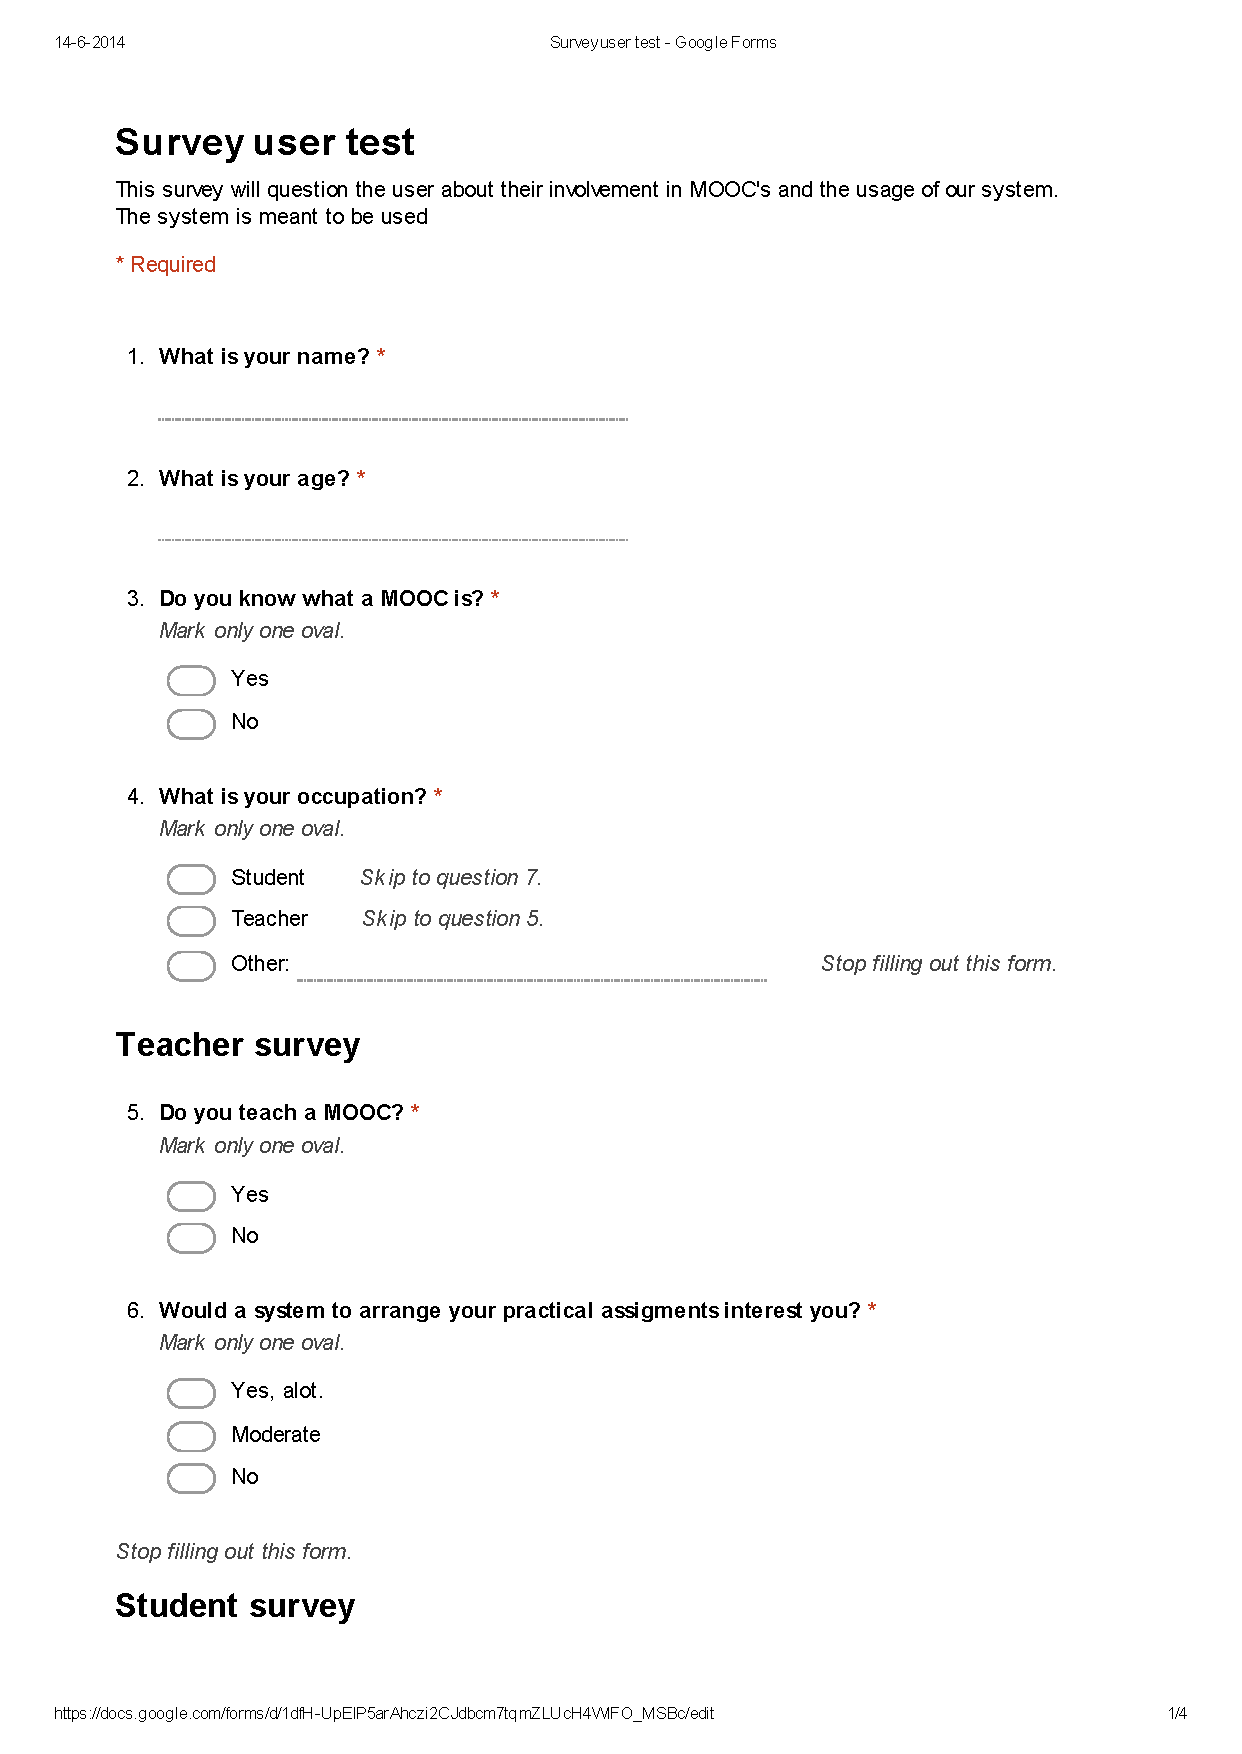
\includepdf[pages=-]{appendix_surveyUserTest_survey.pdf}

\chapter{Appendix E - User test data}
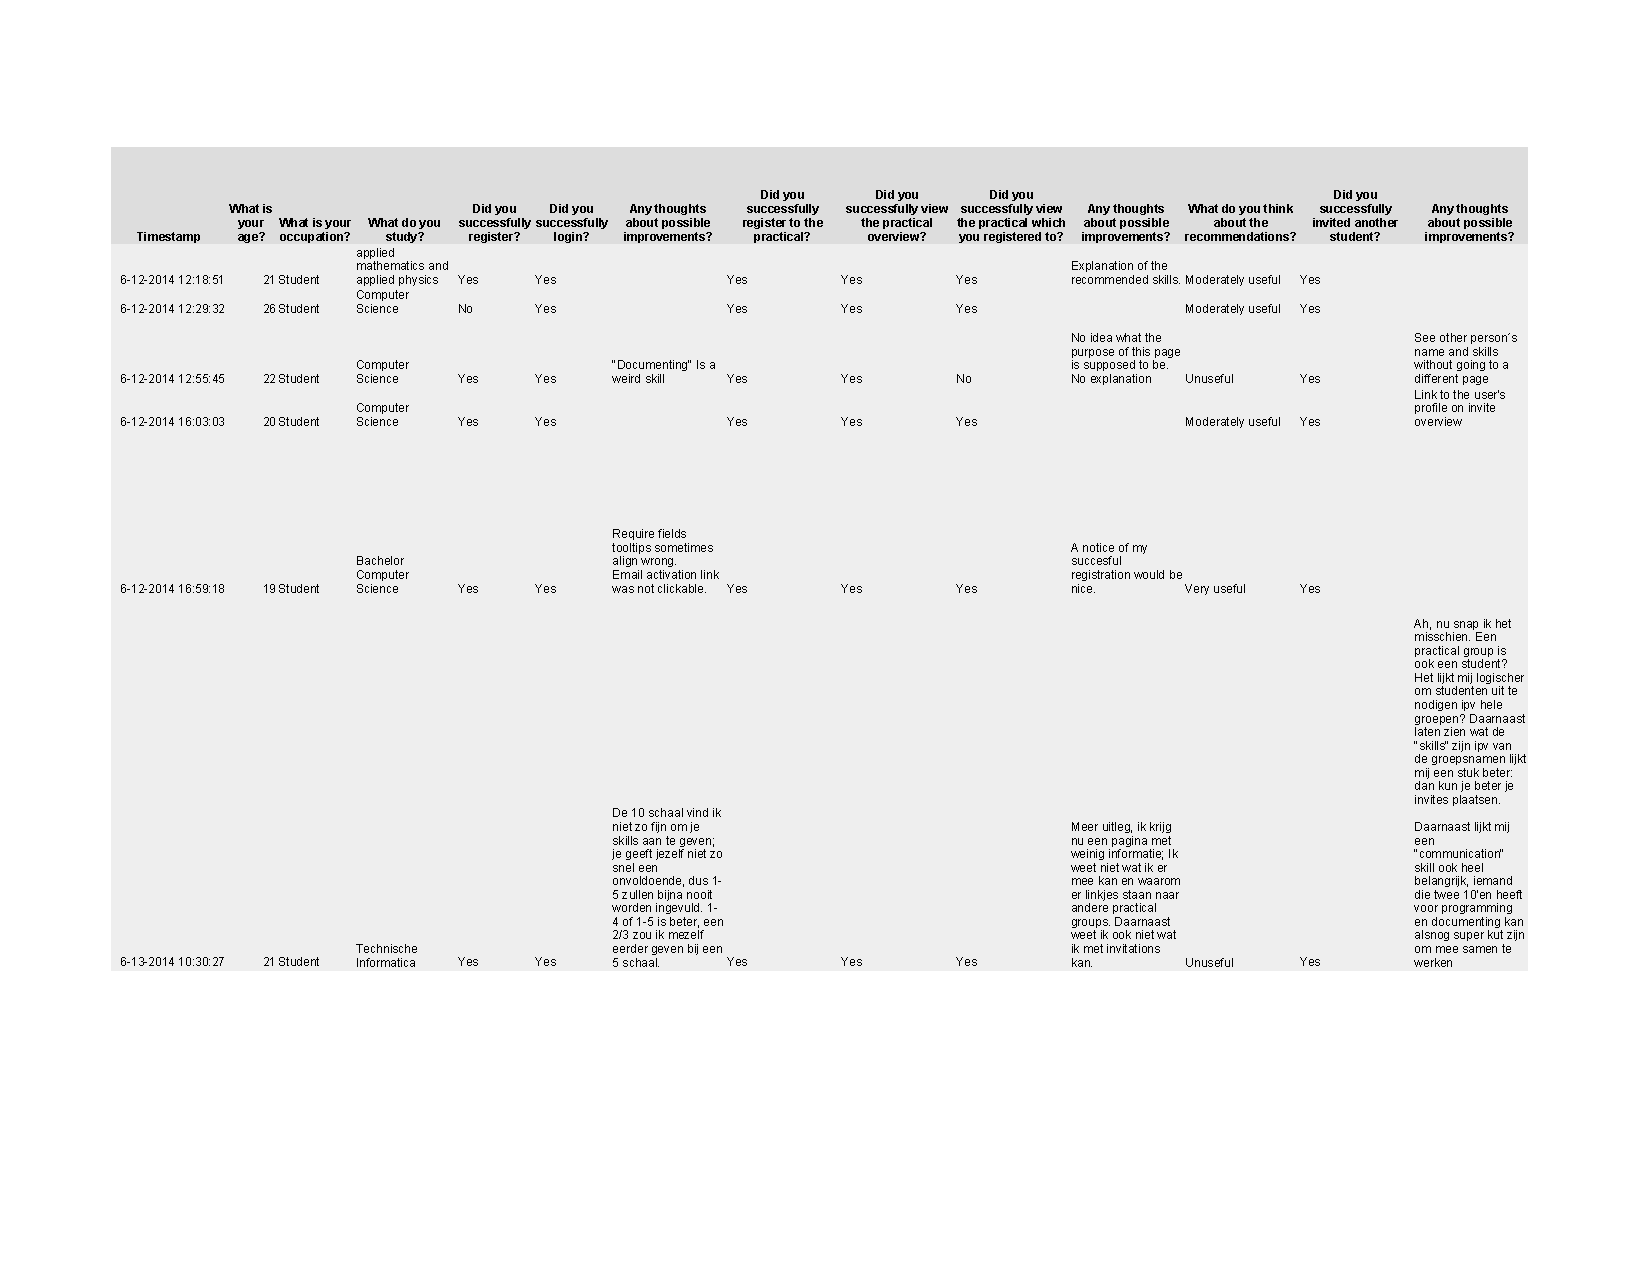
\includepdf[landscape=true,pages=-]{appendix_survey_user_test_data.pdf}

%\includepdf[pages={2-}]{plan_of_approach.pdf}
%\input{"../Plan of Approach/Plan of Approach"}

\bibliographystyle{plainnat}
\bibliography{references}

\end{document}

